\chapter{RyR models}
\label{chap:ryr-models}

This chapter focus on modeling RyR (Chap.\ref{chap:ryan-ryan-recept}).

\section{Overview}

Early RyR computational models assume only cytosolic $\Ca$ plays a role in
regulating RyR channel gating. 

Due to many experimental data that suggest SR lumenal $\Ca$ also regulate RyR
gating \citep{gyorke1998, ching2000}, newer computational models incorporate
lumenal $\Ca$ into the gating of the RyR channels. However, the lumenal $\Ca$
doesn't directly affect the gating but via CSQ , triadin (TRD) and junctin-2
(JCN-2) complex \citep{Gyorke2004, Gyorke2004a}. So, some computational models
incorporate CSQ into the gating of RyR \citep{Lee2008, tania2010}.  \sout{It is
suggested that CSQ inhibit (enhance) RyR activity at low (high) SR $\Ca$ load
through its association (disassociation) with RyR} (not correct)
(Sect.\ref{sec:RyR_CSQ_Triadin_Junctin}). Nevertheless, the precise molecular
mechanism is still elusive.

\section{New papers}

\citep{uehara2002, zucchi1997} 

\section{quark, sparks, waves}
\label{sec:calcium-release-RyR}

The three levels of $\Ca$ releases via RyR in the heart are given as follows.
The $\Ca$ release from the opening of a single channel is known as {\bf quark}
\citep{brochet2011}, while the $\Ca$ release from multiple channel opening is
known as {\bf sparks} which is a local transient restricted to clusters
containing several RyRs \citep{Cheng1993Calciumspark}.

Finally, when many release sites are activated, it causes a global $\Ca$
transient that leads to $\Ca$ wave propagating throughout the cell
\citep{cheng1996csc}.  Chap.\ref{chap:calcium_waves_RYR} discusses
modeling of calcium waves.


\section{Allosteric coupling}
\label{sec:allosteric-coupling-RYR}


\begin{figure}[hbt]
  \centerline{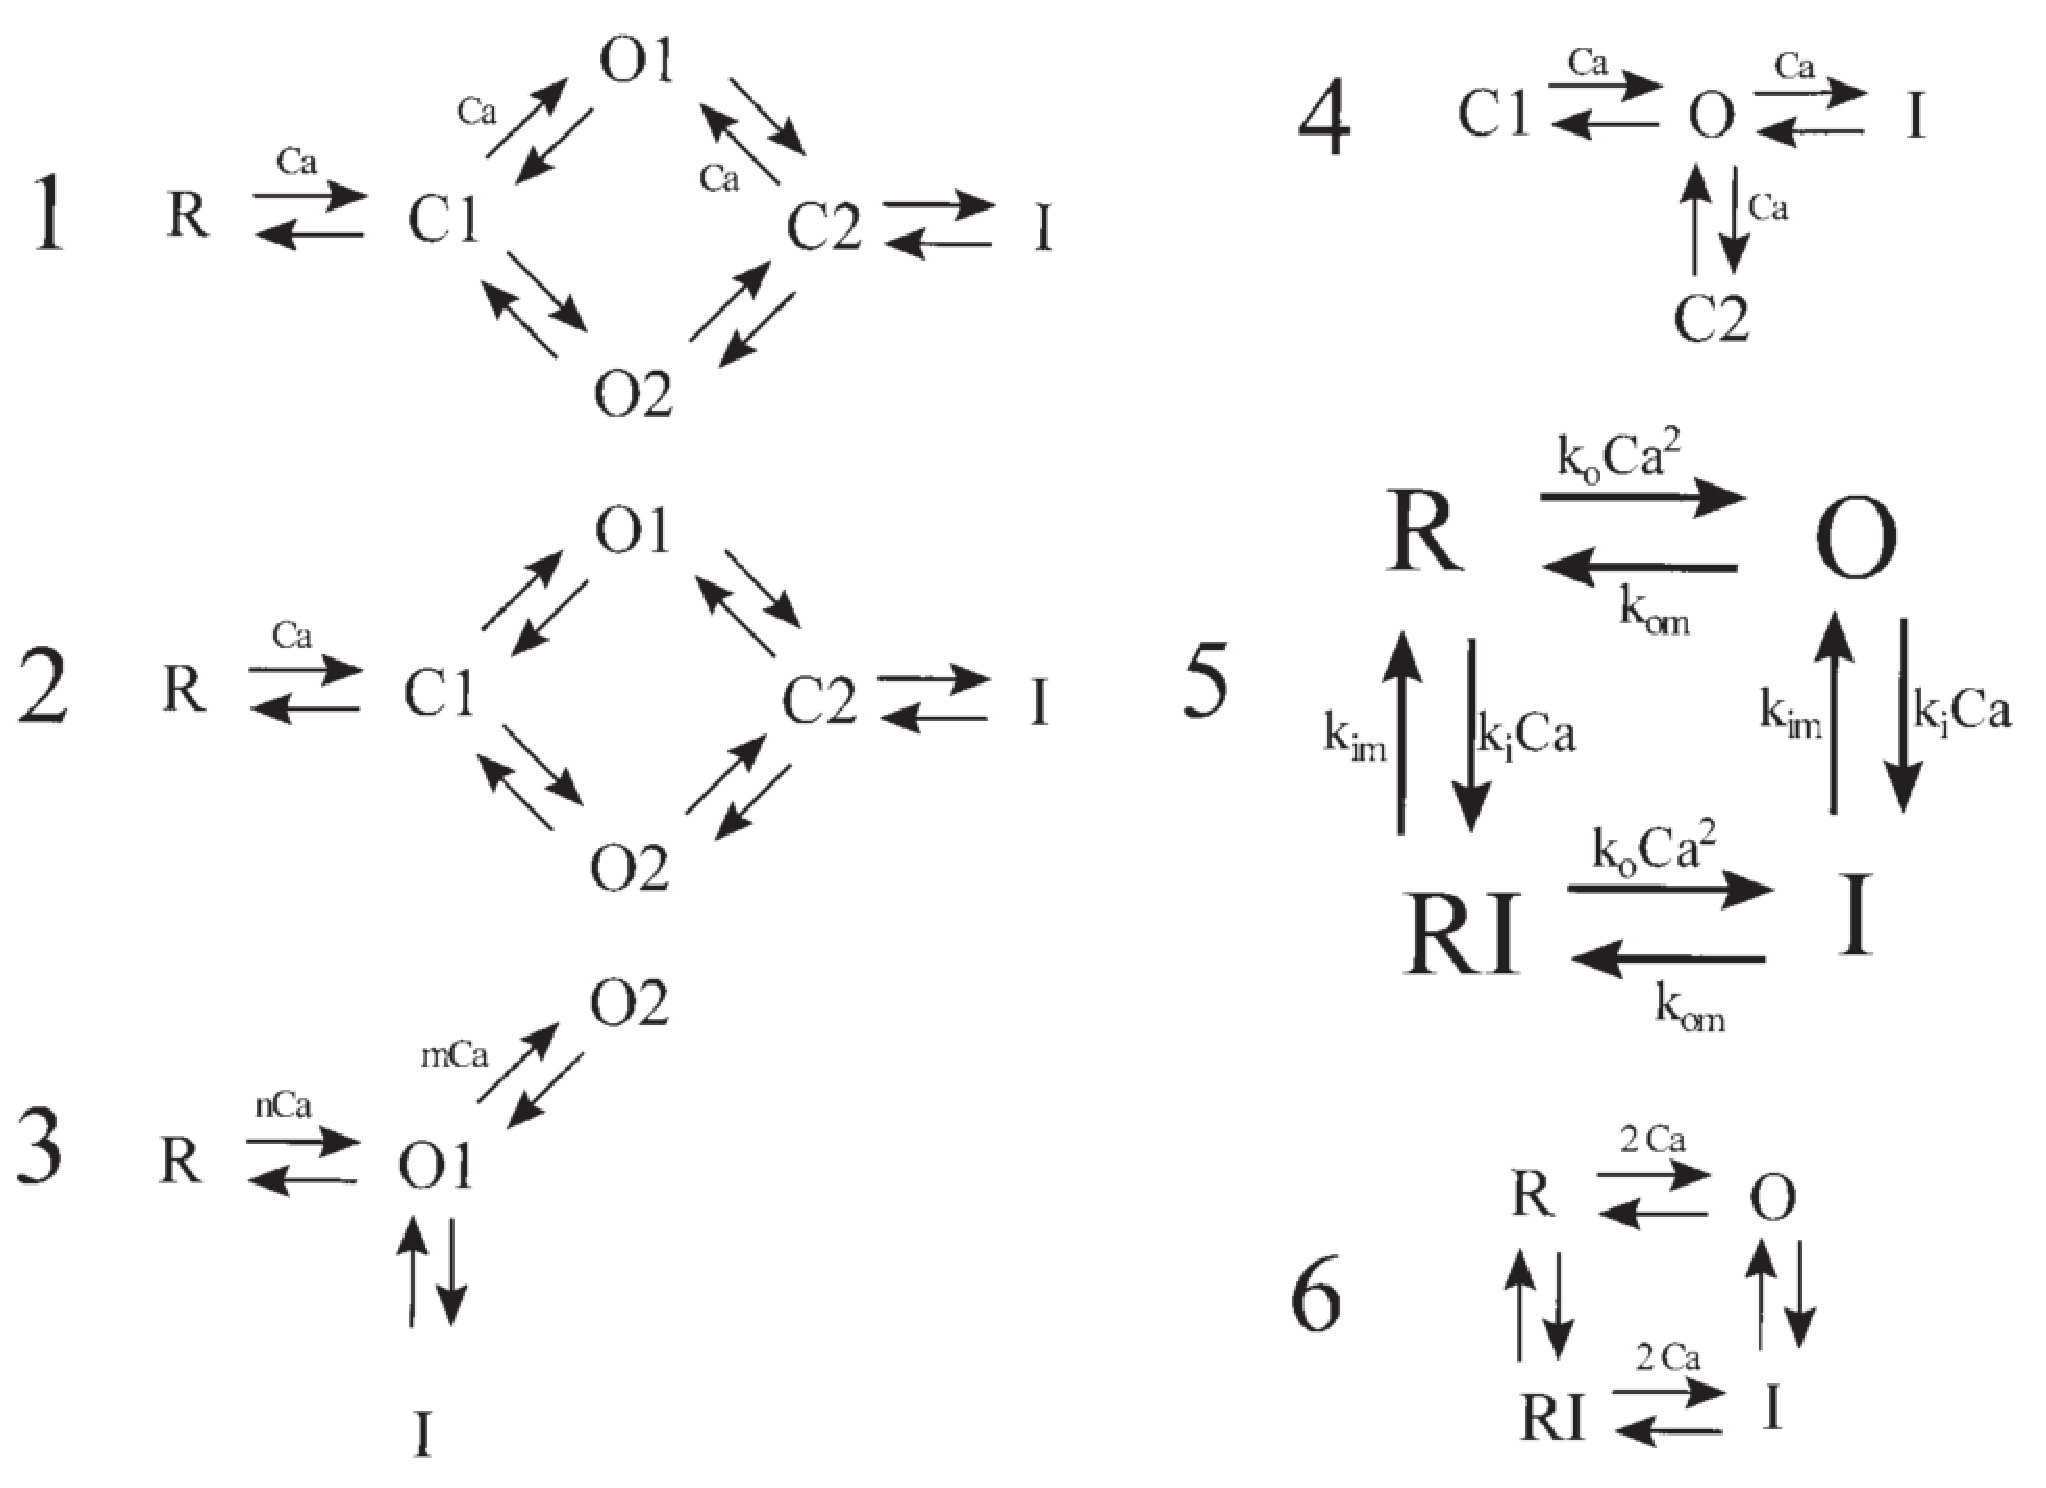
\includegraphics[height=5cm,
    angle=0]{./images/RyR_schemes.eps}}
  \caption{Different RyR schemes derived from experimental data}
\label{fig:RyR_schemes}
\end{figure}

Allosteric interaction is discussed in Sect.\ref{sec:allosteric-coupling}. With
Ryanodine Receptor (RyR), there are evidences that FKBP12 bind to RyR1 (in
skeletal muscle) and FKBP12.6 binds to RyR2 (in cardiac cells) as allosteric
coupling by modifying the sensitivity of the channel to calcium. 

However, in contrast to the clear 'allosteric' effect of FKBP12 on RyR1, the
effect of FKBP12.6 on RyR2 is controversial in early days.~\citep{timerman1993}
shown that removal of FKBP12.6 from canine produced no appreciable effect on the
sensitivity of the RyR2 to $\Ca$.~\citep{Kaftan1996} shown that FKBP12.6
stabilize the closing state of RyR2 and improving allosteric coupling between
RyR, i.e. removal it will increase the opening probability and increase the
randomness in the opening/close thus reducing the current amplitude via the
channels.

As RyR2 is a tetramer with 4 subunits, there are two scenarios: (1) FKBP12.6
couple the subunits to avoid sub-conductance states, (2) FKBP12.6 couple the
neighboring RyRs to stabilize the closing states. Different models examines one
or both of the two different scenarios. Models use the first hypothesis
(intra-receptor coupling): \citep{wang2005ecc}. Models use the second hypothesis
(inter-receptor coupling): \citep{stern1999lcm, sobie2002tcas, williams2011}.
\textcolor{red}{Even though it's suggested that both should give the similar
qualitative form when varying the coupling strenghts, the relative importance of
intra- versus inter- coupling remains to be resolved}.


Using computational model, \citep{stern1999lcm} has demonstrated that single
channel gating derived from planar lipid bilayer experiments, e.g.
Fig.~\ref{fig:RyR_schemes}, failed to produce stable EC coupling if we consider
single channel gating individually. The result is in agreement with Kaftan {\it
et al.}'s study.  Thus, in an RyR cluster, arranging in a lattice array, it's
believed that there is an allosteric interaction between the large foot
processes of adjacent RyRs. The question is how we model {\bf allosteric
coupling} using a mathematical formula? The coming section will describe in
details different approach, including {\it ad-hoc}-based formula.

\begin{figure}[hbt]
  \centerline{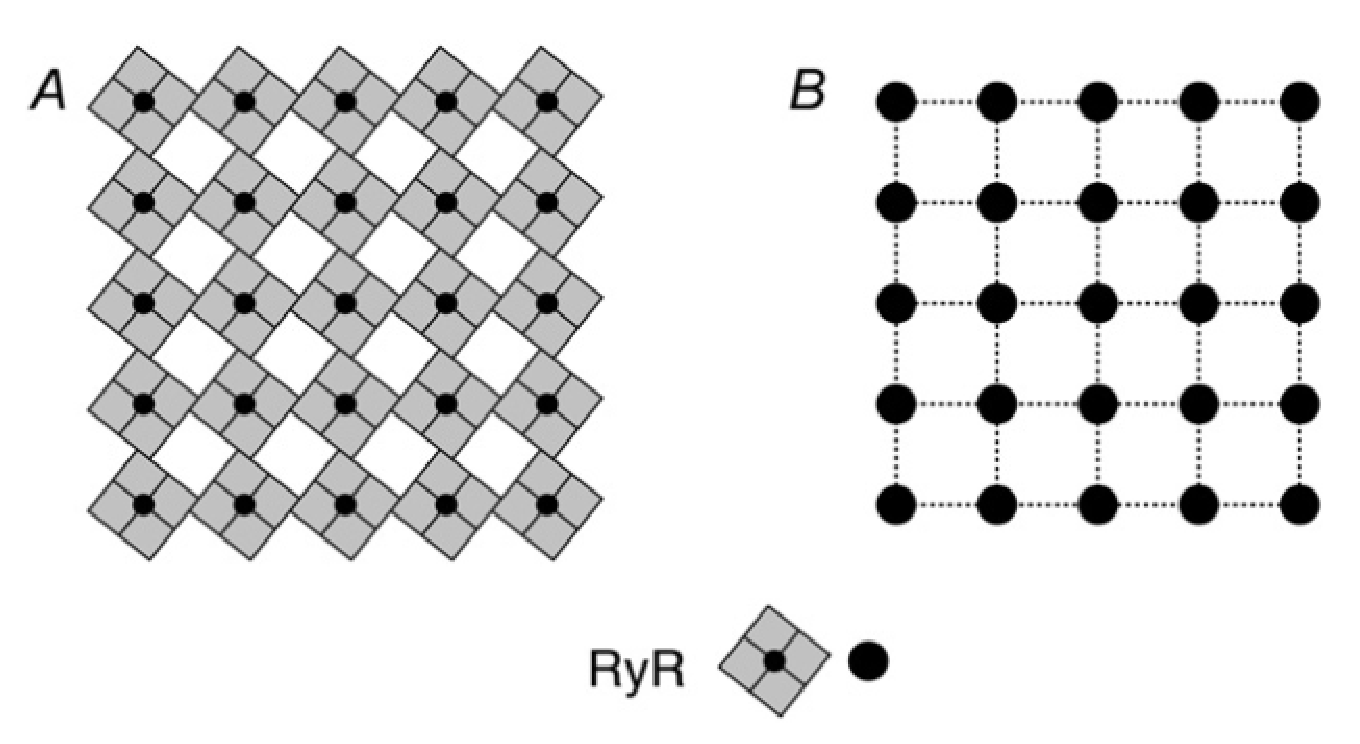
\includegraphics[height=4cm,
    angle=0]{./images/RyR_schematic.eps}}
  \caption{Crystal arrangement of RyR in a cluster~\citep{groff2008}}
\label{fig:RyR_schematic}
\end{figure}

From the underlying biological point of view, how can we explain this mechanism?
Given that the large foot process of the RyR appear anatomically in contact, a
reasonal explanation is that when an RyR open, its foot process interacts with
the foot process of nearest neighbor RyRs, enhancing the stability of the
inactivated state of neighboring RyRs \citep{stern1999lcm}. The foot has an
important, though unknown, function. In a planar setting of RyR, a single RyR is
assumed to have maximum 4 neighboring RyRs, Fig.~\ref{fig:RyR_schematic}. Such
allosteric interaction may be a function of foot process and lattice array (i.e.
dense 2D crystalline array).  The pore-to-pore interchannel distance is 30 nm.
\textcolor{blue}{Recent evidences suggested that RyRs are not arranged in a
densed bilayer setting, but scatter in smaller cluster with arbitrary layout.
This may affect to how we model allosteric coupling. However, there hasn't been
any studied to model such hypothesis and how much its affect to the EC
coupling}.

Now, we describe how allosteric coupling effect is incorporated into RyR model.
At first, the transition rate of the single channel in isolation $k_{ij},
k_{ji}$ from one state to another is described as follows
\begin{equation}
  \label{eq:1123}
  \ce{S_i <=>[k_{ij}][k_{ji}]S_j}
\end{equation}

The allosteric coupling effect is defined via an allosteric coupling
factor $\chi_{ij}$, and is added into the model to produce robust local
stability. So, the new transition rate is $K_{ij}=k_{ij}\times \chi_{ij}$.
\begin{equation}
  \label{eq:1216}
  \ce{S_i <=>[k_{ij}\chi_\ij][k_{ji}\chi_\ji] S_j}
\end{equation}

\citep{wang2004} showed that a spark is the result of 1 RyR (12\%), and multiple
of RyR upto 8 (88\%). They excluded the possibility that a spark is the result
of entire array 100 RyRs or a fixed number of RyR2. In an array, the multiple
opening of RyR2 reduce the spark duration. The quantal of calcium release via a
single RyR channel was expected 1.22 pA. In lipid bilayers, a single RyR {\it in
vitro} under quasi-physiological conditions carries 0.5-1.4 pA, depending on
exact ionic conditions. So, the array-based behavior is
important in shaping $\Ca$ spark dynamics \citep{wang2004}. \citep{Liang2009}
predicted that RyR array has dynamic coupling {\it in vivo}.

\subsection{Stevens (1978)}

When studying the gating of $V_m$-dependent ion channel, \citep{stevens1978}
concluded that transition rates is an exponential function of $V_m$ over a
limited voltage range. Also, Stevens assumed that there are two major
conductances, open and closed. 

In general, a protein with $n$ conformations: 1,2,\ldots,k,\ldots,$n$. Let
$P(k)$ be the probability for finding the $k$ conformation at equilibrium. With
$N$ channels in total on the membrane, the average conductance $g(t)$ is given
by
\begin{equation}
g(t) = N \sum_{k=1}^n	\gamma_k P_k(t)
\end{equation}
with $\gamma_k$ is the conductance at conformation $k$. NOTE:
$\sum_k\gamma_kP_k(t)$ is the average conductance for one channel. 

The probability for each channel having conformation $k$ at time $t$, $P_k(t)$,
is governed by the so-called {\bf master equation}.
\begin{equation}
\frac{dP_k(t)}{dt} = \sum_j	\alpha_{jk}P_k(t) - \sum_j \alpha_{kj}P_k(t)
\end{equation}
This requires the knowledge of transition rate from one conformation to another,
i.e. the transition rate $\alpha_{ij}$ from conformation $i$ to conformation
$j$. NOTE: $\alpha_{ij}(V_m)$ is a function of $V_m$.
\begin{equation}
\alpha_{ij}(V_m) = \eta \exp\left( -U_{ij}(V_m)/(k_BT) \right)
\end{equation}
with $\eta$ is the attempt rate, $U_{ij}(V_m)$ is the free energy difference
$E_{ij}-E_{il}$ with $l\ne k$.

The free energy of the conformation $k$ can be calculated from the partition
function $Z_k$, i.e. $U_k = -\frac{1}{k_BT}\frac{\partial \ln Z_k}{\partial}$. 
\begin{equation}
Z_k = \sum_{r\in \{k\}} e^{-w_r(V_m)/(k_BT)}
\end{equation}
with the sum indicates the sum extends over all states that constitute the
conformation $k$. Each arrangement, consistent with the integrity of channel
structure (the $r$-th state) has the energy $w_r(V_m)$. NOTE: The energy barrier
that separates the two different conformations is appreciably larger than the
energy barriers between the states constituting any particular conformation. 

\begin{framed}
Bond and group dipole moments are on the order of 1D, i.e. a single bond can
provide, in a 100 kV/cm field, energies that amount to only about 1\% of $k_BT$.
One electronic charge moving about 25$\AA$ in a 100 kV/cm field
changes energy by 1$k_BT$ unit. 
\end{framed}

\subsection{Marks-Jones (1992) - DHPR}
\label{sec:DHPR_Marks1992}

\citep{marks1992} studied the effect of dihydropyridine (DHP) $\Ca$ channels
under the absence and presence of DHP. A modified Monod-Wyman-Changeux (MWC)
model was suggested for channel activation. MWC model was first suggested for
hemoglobin. It was suggested that depolarization induces small, local
conformational change in the channel protein, presumably movement of the S4
helices, the local change can facilitate channel opening which might be a global
conformational change, i.e. the opening is assumed to be voltage-independent.
So, the movement of the voltage sensor is analogous to ligand binding, and open
and closed states correspond to the active (R) and inactive (T) states of the
hemoglobin. A 6-state model is suggested, Fig.\ref{fig:DHPR_Marks1992}(A) in
which the voltage sensors are assumed to be identical. The channel is assumed to
be tetramer with 4 voltage sensors. This scheme is determined by 4 parameters
which are functions of $V_m$.
\begin{equation}
\begin{split}
k_C &= A.e^{(V_m/V_s)} \\
k_{-C} &= B.e^{(-V_m/V_s)}
\end{split}
\end{equation}
with $A,B$ are rate constants at 0mV, $V_s$ is inversely proportional to the
equivalent charge moved across the membrane field between a state and a
transition state. So, the microscopic voltage dependence of the model is
determined by a single parameter $V_s$, the amount of charge moved by one
voltage sensor.

Under the assumption that DHPR agonists act as allosteric effectors to stabilize
the open states of the channel, the mode-gating is a way of modelling the
allosteric effect. At each closed state, the channel can switch to open which is
voltage-independent and theoretically possible with any number of voltage
sensors, but are much more likely with an increasing number of voltage sensors
in the + positions, Fig.\ref{fig:DHPR_Marks1992}(B).

\begin{figure}[htb]
  \centerline{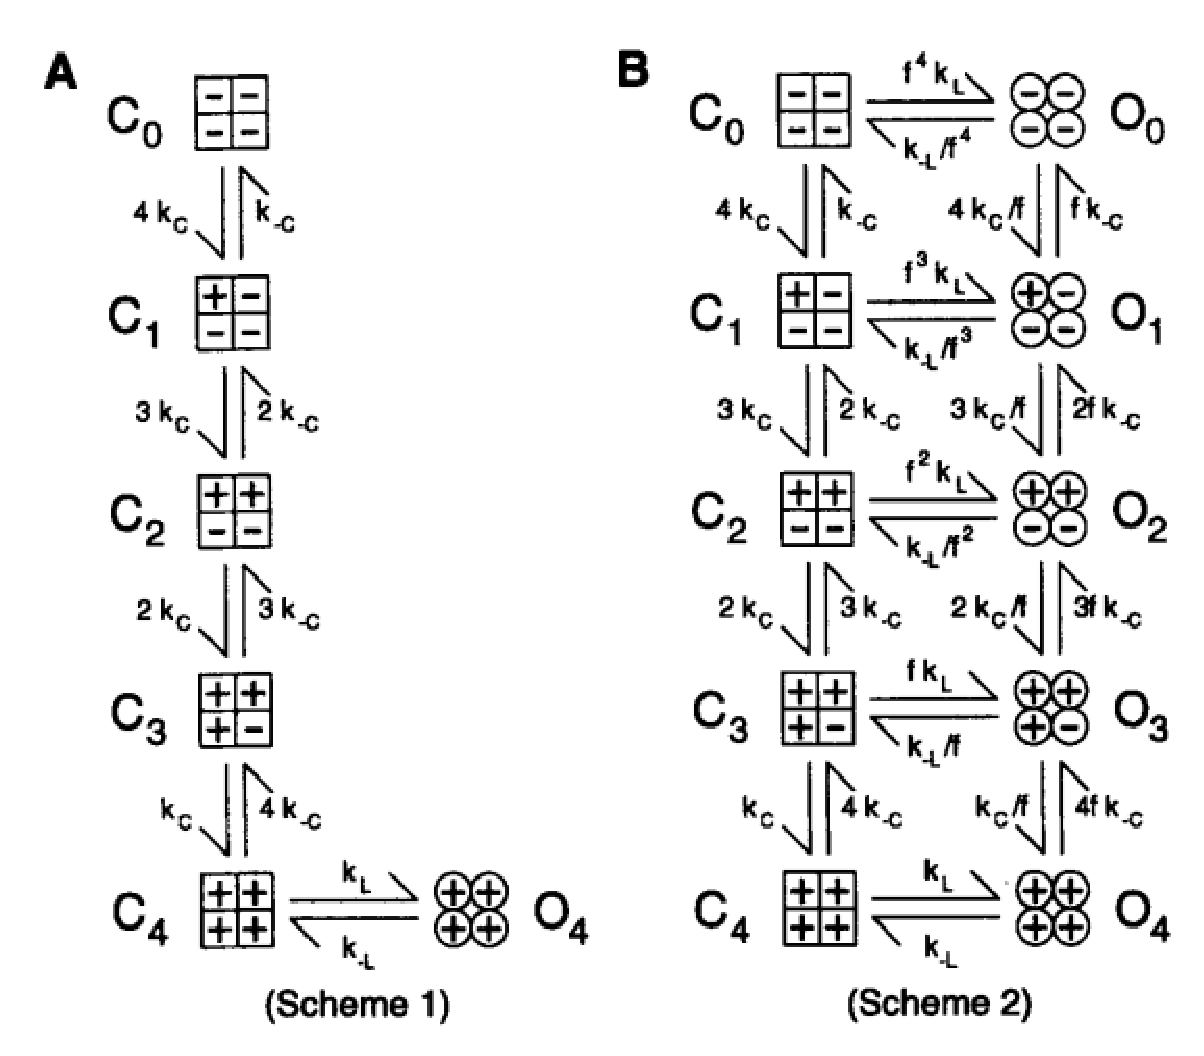
\includegraphics[height=5cm]{./images/DHPR_Marks1992.eps}}
  \caption{(A) Linear 6-state model, with vertical transitions reflect movement
  of voltage sensor, and horizontal transition reflects channel opening which is
  voltage-independent. (B) MWC model with allosteric proteins. The factor $f$ is
  allosteric factor. Also, the voltage sensors move from the - to + positions
  more readily when the channel is in the open state \citep{marks1992}}
  \label{fig:DHPR_Marks1992}
\end{figure}

Even though MWC model incorporating allosteric effect is complex, with 10 states
and 26 rate constants, the rate constans are determined by relatively few free
parameters, given the cyclic nature of the model and the assumptions of
symmetry. There are 5 parameters $(k_c, k_{-c}, k_L, k_{-L}, f)$. This is one
additional parameter than Scheme 1, i.e.  $f$ defines the voltage dependence.
So, it's assumed that DHP agonists act as allosteric effectors to stabilize the
opening the open state, similar to the role of 2,3-diphosphoglycerate to T-state
of hemoglobin. Here, the allosteric factor is formulated with a beta
distribution
\begin{equation}
f(x) = x^{(a-1)}(1-x)^{(b-1)}
\end{equation}
with $a=k_L\tau$, $b=k_{-L}\tau$; $x$ is the current amplitude (on the scale
0=closed, 1=open); $k_L, k_{-L}$ are opening and closing rates; and $\tau$ is
the cutoff frequency of the filter.

The main challenge is fitting the model. The sequence used for determination of
the model parameters is given as follows. The rate constants for channel opening
$k_L, k_{-L}$ are determined primarily by channel gating during bursts
($L=k_{-L}/k_L$ is equilibrium constant of closing transition).
Closed-closed transitions $(k_C, k_{-C})$ depends in part on the steady-state
activation curve (which determines the ratio
$K_C=k_{-C}/k_C=\exp\left[-\frac{V_m-\bar{V}}{4K}\right]$ equilibrium constant
among closed states, and voltage dependence). The shift in the activation curve
by DHP agonists set the factor by which $k_L, k_{-L}$ are changed. The factor
$k$ which strongly influences the cooperativity is not directly measured from
the experimental data.


\subsection{Rios-\ldots-Gonzalez (1993)}

This is an extension to the work described by \citep{marks1992}
based on Monod-Wyman-Changeux model of allosteric transition in
hemoglobin (Sect.\ref{sec:DHPR_Marks1992}). For each voltage-sensor molecule:
$\ce{r <=>[k_C][k_{-C}] a}$, the two-state transition is governed by Boltzmann
distribution so that $P_a/P_r = \exp[(V_m-\bar{V})/(4K)]$. So, the rate constant
can be described by the exponential rate that assume symmetric barrier
\begin{equation}
\begin{split}
k_C &= 0.5 \alpha . \exp\left[(V_m-\bar{V})/(8K)\right] \\
k_{-C} &= 0.5 \alpha . \exp\left[-(V_m-\bar{V})/(8K)\right] \\
\end{split}
\end{equation}
with $\alpha$ is the inverse of the time constant at $V_m=\bar{V}$.

At rest, all the sensor molecules are in state $r$ ($\bar{V}\approx -40$mV).
This requires $k_L \ll k_{-L}$, so the typical values for simulation is
$k_L=0.003, k_{-L}=1000$ ms$^{-1}$.


\subsection{Stern {\it et al.} (1999)}
\label{sec:RYR_Stern1999}

  \begin{figure}[htb]
    \centerline{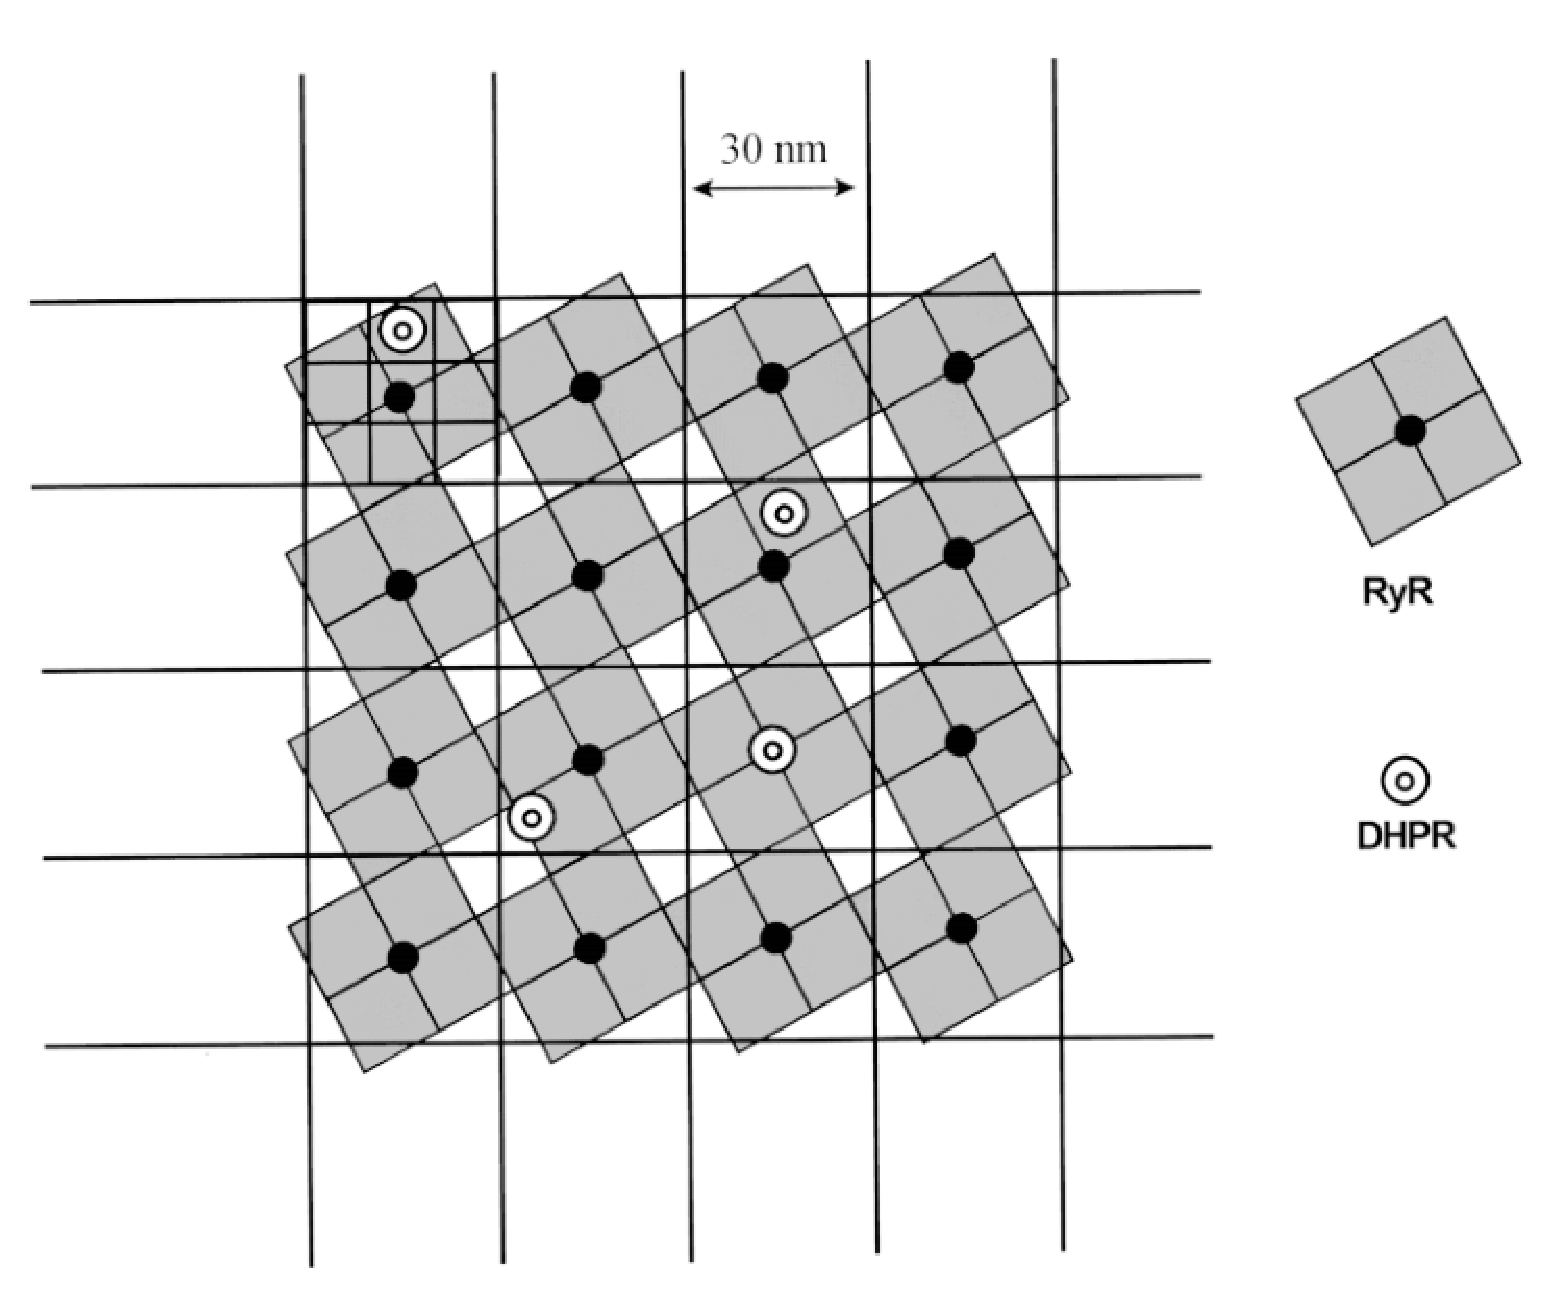
\includegraphics[height=5cm]{./images/RyR_Stern1999.eps}}
    \caption{The paracrystallized organization of RyRs
    in the dyad. DHPR were located randomly on mesh
    squares of size 10nm, while each RyR spans 30nm}
    \label{fig:RyR_Stern1999}
  \end{figure}

The existence of allosteric interactions between large foot processes of
adjacent RyRs, which appear anatomically in contact, was assumed. Based on the
arrangement given in Fig.\ref{fig:RyR_Stern1999}, it's assumed that each RyR has
maximum 4 neighbors ($m=1...4$). To satisfy the constraint of microscopic
reversibility, the interactions were specified in the form of free energies
interaction between neighboring RyRs. To determine the transition $K_{ij}$ from
state $i$ to state $j$ of a single RyR, the allosteric effect from neighboring
channels are examined ~\citep{stern1999lcm}. This effect from the neighbor
channel $m$ is represented in the form of allosteric interaction energy
$E_{js_m}$, i.e. the addition of free energy experienced by the RyR from its
neighbor $m$ in state $s$ for the current channel to jump to state $j$. If the
energy is positive, the energy barrier is thus lower or making the channel
easier to jump to state $j$; and conversely if the energy is negative, the
energy barrier is increased. It's zero if the neighbor $m$ is absent from the
array. For microscopic reversibility (the products around the loop of forward
and reverse rates be equal), $E_{js_m}=E_{s_mj}$.

\begin{equation}
\ce{i <=>[k_{ij}\chi_{ij}][k_{ji}\chi_{ji}] j}
\end{equation}

So, the transition should be increase/decrease respectively, by multiplying with
a factor, which can be formulate as
\begin{equation}
    \label{eq:1129}
    \chi_\ij(s_m) =
    \exp\left(-\frac{\eta_{js_m}E_{js_m}-\eta_{is_m}E_{is_m}}{k_BT}\right)
\end{equation}
with $\eta$ are the factors that ``partition'' the allosteric effect  between
the forward (i to j) and backward (j to i) transitions, i.e the
splitting coefficient $\eta_{ij}=1-\eta_{ji}$. To remove the effect of scaling
by energy unit, we divided them by $k_BT$.

So, between the two state $i$ and $j$, the difference
$\eta_{js_m}E_{js_m}-\eta_{is_m}E_{is_m}$ will tell how the allosteric energy
help state channel to energetically reach state $j$ or keeping in state $i$.
If the difference is negative, then the energy required to jump to state $j$ is
lower than to jump to state $i$ or we can say state $j$ is more susceptible.
This requires an increasing in the transition rate, or the exponential term
should be greater than one, i.e. the negative sign in the exponential term is
requires.
$\eta_{js_m}E_{js_m}-\eta_{is_m}E_{is_m}<0$ will make $\chi_\ij> 0$.
\textcolor{blue}{The more negative of
  $\eta_{js_m}E_{js_m}-\eta_{is_m}E_{is_m}$, the more positive of $\chi_\ij$ or
 the more susceptible in transition from state $i$  to $j$}.

  % If we assume that the allosteric interactions make the destination
  % (state $j$) more energetically favorable, it means that
  % $n_{js_m}E_{js_m}$ is smaller than $n_{is_m}E_{is_m}$, or the
  % subtraction is negative. That's why we need to add a negative sign
  % in the front to make the term $\exp(-(...))$ greater than one. This
  % will increase the transition rate from $i$ to $j$.

  To consider all possible neighbors, with maximum four neighbor, we
  sum them up and then take exponential
  \begin{equation}
    \label{eq:1070}
    \chi_\ij = \exp\left(-\sum_{m=1}^4\frac{\eta_{js_m}E_{js_m}-\eta_{is_m}E_{is_m}}{k_BT}\right)
  \end{equation}

  Finally, the rate constant is
  \begin{equation}
    \label{eq:1071}
    K_{ij} = k_{ij}
    \exp\left(-\sum_{m=1}^4\frac{\eta_{js_m}E_{js_m}-\eta_{is_m}E_{is_m}}{k_BT}\right)
  \end{equation}
  NOTE: This is the right notation, not the one being used in Stern
  {\it et al.}  paper.

\begin{framed}
  From reaction rate theory point of view, $\eta$ is the weighting
  factor (or partition contribution of the allosteric energy) for the
  initial (``reactants'') and final (product) states.  In general,
  each source of allosteric energy can have its own weighting
  factor. However, to avoid the proliferation of parameters, we can
  assume that it's the state transition is important, not the individual
  channel. Or we can say ``regardless of the individual channel, the partition
  is the same for the same state transition'', i.e.
  $\eta_{js}=\eta_{is}=\eta_{ij}$, with $n_\ij=1-n_\ji$. Then

  \begin{equation}
    \label{eq:1130}
    K_{ij} = k_{ij}
    \exp\left(-\eta_{ij}\frac{\sum_{m=1}^4(E_{js_m}-E_{is_m})}{k_BT}\right)
  \end{equation}
It's reasonable that $\eta$ should lies between 0 and 1, but this is not
required. By default, $\eta=0.5$ was assumed, i.e. $n_{ij} = n_{ji}$.
\end{framed}

\begin{figure}[hbt]
  \centerline{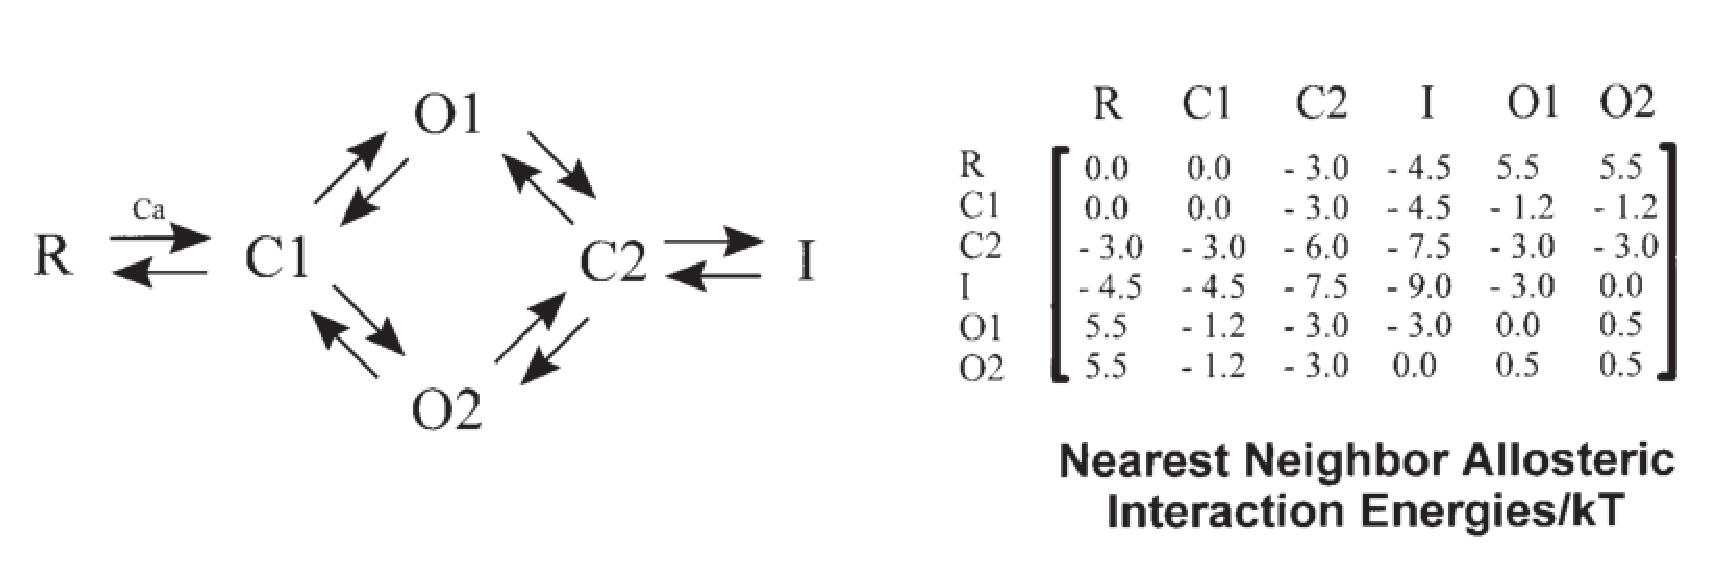
\includegraphics[height=3cm,
    angle=0]{./images/RyR_Zahradnikova1996_Stern1999.eps}}%Zharadnikova_RyR.eps
\caption{RyR gating scheme with one $\Ca$ binding
site~\citep{zahradnikova1996}, and the allosteric coupling
energies\citep{stern1999lcm}}
\label{fig:RyR_Zharadnikova1996}
\end{figure}

Based on the sample model of slow inactivation and single calcium
binding site in Fig.~\ref{fig:RyR_Zharadnikova1996}, binding one calcium to the
channel in state R, it can open the channel if the channel was in isolation.
However, to move the channel from state C1 to O1 or O2 when it is surrounded by
resting channels, it would be much harder due to energy barrier caused by
allosteric coupling. When it have more of its neighboring in calcium-bound
state, then the energy barrier is decreased so that RyR can open. The important
point is that for this strategy to work, the underlying single-RyR gating must
have a closed state with calcium-bound. ~\citep{stern1999lcm}
derived two important points to choose allosteric interaction
energies:
\begin{enumerate}
\item to produce local stability,
  \textcolor{red}{the forward rate of inactivating transition need to
    be increased}. An example is to use $E_{ij}=-E/4$ if one of the two
    states in inactivated and $-E/2$ if both are, so that adding this
    allosteric energy will contribute $-E$ to the free energy change
    associated with any transition to inactivated state of a channel
    with 4 neighbors.

  \item to produce global stability,
    \textcolor{red}{multiple-calcium binding site need to be assumed}.
    For single calcium binding site, we add a large, positive
    allosteric contact energy between the RyR in open state and its
    neighbor in closed state. If we
    consider multiple-calcium binding site, then there is a chance
    that the neighbors have switched to close state, which decreases
    the energy barrier. So, the conclusion is that for this strategy
    to work, we need a model of multiple-calcium binding site, and it
    needs to occur before any channel can open. However, it doesn't
    mean that binding a single calcium cannot open the RyR; it's just
    very rare. This small likelihood provides a chance that single RyR
    openings can trigger the whole array.
\end{enumerate}

The choice of allosteric energies should not be considered unique or optimal.
The choice of allosteric energies, while it produces positive cooperativity
between RyRs, does not give rise to the perfect synchronization of opening and
closing of coupled RyRs observed by \citep{marx1998}. It seems that allosteric
interaction is not required for producing sparks, as removing FKBP12.6 doesnot
abolish sparks \citep{mccall1996}. Maybe, allosteric interactions affect the
frequency of sparks, duration and induce global calcium oscillations
\citep{xiao1997}.


\subsection{Sobie {\it et al.} (2002)}
\label{sec:RYR_Sobie2002}

Experimental data have shown that spark termination is independent
from spark triggering, i.e. the spark duration can be short or
long~\citep{cheng1993cse}. Besides, a small influx of $I_\Ca$ (0.5pA,
0.5ms) can trigger a spark with $>98\%$ fidelity.

Using a minimal (mean-field) approach, i.e. disregard the location of
individual channels and only examine the number of channel in a given
state, ~\citep{sobie2002tcas}
(Sect.~\ref{sec:sobie2002_jafri}) proposed an ad-hoc coupling (or
``cooperativity'') factor. The coupling factor is defined based on the number
of open channels, e.g. using a 2-state RyR model, the two coupling
factors are

\begin{equation}
  \label{eq:1134}
  \begin{split}
    \CF_\open &= 1 + \frac{N_\open + 1}{N}\\
    \CF_\close &= k_\text{coop}\left[1 + \frac{N_\open + 1}{N}\right]\\
  \end{split}
\end{equation}
with $N=N_\close+N_\open$ is the number of RyRs in the dyad;
$k_\text{coop}$ is used as a scaling factor to simulate the change in
the strength of inactivating coupling between RyRs (equal to unity in
control conditions).
\begin{equation}
  \label{eq:1215}
  \ce{ C <=>[k^+\chi_C][k^-\chi_O] O}
\end{equation}
with $\chi_C = \CF_\open$ and $\chi_O=\CF_\open$.

Each neighboring channel in the same state reduce channel's energy by $E_j$,
whereas each channel in the opposite state increases the energy by $E_j$. NOTE:
The activation energy for each transition is assumed to be equal to 1 ($k_BT$),
and \citep{sobie2006} chose $Ej=0.8$($k_BT$). Strong coupling cause the
steady-state $P_o$ vs. $[\Ca]_\ds$ becomes very steep. This causes RyR in the
cluster very stable at closed state when $[\Ca]_\ds$ is low enough, but become
very high when the calcium pass a certain threshold. So, it may explains the
reason that PKA phosphrylation of isolated RyRs cause an increase in the peak
channel $P_o$ after rapid jumps in $[\Ca]_\ds$, but little increase at
$[\Ca]_\ds=100$ nM \citep{valdivia1995}.

\begin{figure}[hbt]
  \centerline{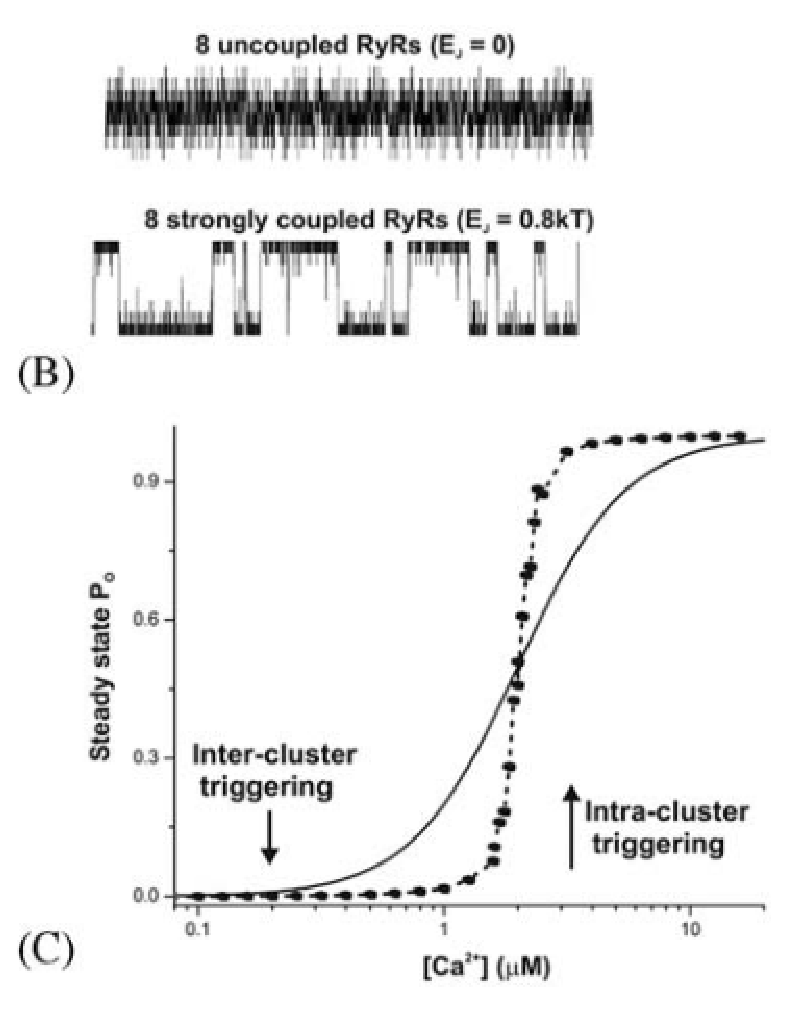
\includegraphics[height=7cm,
    angle=0]{./images/RyR_coupling_Sobie2006.eps}}
  \caption{Strong energetic coupling ($E_j=0.8$) causes $P_o$ vs. $[\Ca]_\ds$
  curve becomes verys steep (dashed line) compared with the relationship for an
  isolated channel (solid line)}
  \label{fig:RyRcoupled_Sobie2006}
\end{figure}


\subsection{Ming-Wall (2005)}

To describe the conformation change of a protein before and after a ligand
binding, a statistical measure that quantifies how close a probability
distribution $p={p_i}$ to a candidate (model) distribution $q={q_i}$ known as
{\bf Kullback-Leibler divergence} (KL) $D_\mathbf{x}$ is used \citep{ming2005}.
Let
\begin{itemize}
  \item $P(k), P(\mathbf{x})$ are equilibrium probability distribution of reaction
rates $k$ and multidimensional configuration $\mathbf{x}$ of the apo-protein
\item $P'(k), P'(\mathbf{x})$ are non-equilibrium probability distribution of
reaction rates $k$ and configuration $\mathbf{x}$ of the ligand-bound protein.
\end{itemize}
The formula is
\begin{equation}
\begin{split}
\bar{D}_k	&= \int_0^\infty dk \left( \log \frac{P'(k)}{P(k)} \right) P'(k) \\
\bar{D}_\mathbf{x}	&= \int_0^\infty d^{3N}\mathbf{x} \left( \log \frac{P'(\mathbf{x})}{P(\mathbf{x})}
\right) P'(\mathbf{x})
\end{split}
\end{equation}
The relation between a protein conformation and its reaction rate is complex.
Due to the limitation in our understanding of protein chemistry, there's
currently no general method for theoretical calculation of $P(k)$ for proteins.
Assuming the rate $k(\mathbf{x})$ is a function of the configuration
$\mathbf{x}$, then
\begin{equation}
P(k) = \int d^{3N} \mathbf{x}P(\mathbf{x}) \delta (k(\mathbf{x}-k))
\end{equation}

$D_\mathbf{x}$ is a non-negative, non-symmetric (it's not a true metric as KL from Q to P
is not the same as KL from P to Q). $k_B.T.D_\mathbf{x}$ is allosteric free-energy, i.e.
the free energy change associated with changing the ligand-free conformational
distribution of the protein to the ligand-bound conformational distribution.

Again, the main question is {\bf how we formulate $\chi_{ij}$?} To satisfy the
microscopic reversibility, the interaction was specified in the form of RyR-RyR
interaction free energy (i.e. $\Delta G^\#$). The conformational distribution
of a protein without the ligand binding is based on Boltzmann distribution and
is given as follows ~\citep{wall2006}
\begin{equation}
  \label{eq:1213}
  P(\mathbf{x}) = Q^{-1} \exp(-\frac{ G(\mathbf{x})}{k_BT})
\end{equation}
with $G(\mathbf{x})$ is the Gibbs free energy of a
protein in conformation $\mathbf{x}$ in the solution at a constant temperature and
constant pressure. $Q$ is the partition function, which relates to the total free
energy $G$ of the protein as
\begin{equation}
  \label{eq:1214}
  G = < G(\mathbf{x})>_\mathbf{x} - TS_\mathbf{x} = -k_BT.\ln Q
\end{equation}
with $< G(\mathbf{x})>_\mathbf{x}$ is the mean free energy, and
$S_\mathbf{x}=-k_B<P(\mathbf{x})\ln P(\mathbf{x})>_\mathbf{x}$ is the entropy of conformational distribution.
If we consider $G'(\mathbf{x})$ as the new Gibbs free energy when a ligand is
bound to, the $\Delta G=G'(\mathbf{x}) - G(\mathbf{x})$ is the change in free
energy.

\subsection{Wang-\ldots-Levine (2005)}
\label{sec:wang-levine2005_RYR}

\citep{wang2005ecc} studied the effect of FKBP12.6 (FK506-binding protein) on
the cooperativity between subunits in the same RyR2. The effect of FKBP12.6 on
the coupling between neighboring receptors has not been studied here. Using
the model, the results shown that the dissociation of FKBP12.6 causing a rise in
RyR leak and concomitantly the reduced SR $\Ca$ content.

Under the absent of FKBP12.6, the channel can exhibits 1/4, 2/4 or 3/4 of the
total channel conductance \citep{brillantes1994}. Thus, they assumed each
subunit in the RyR tetramer can conduct $\Ca$ by itself, upon the binding of one
calcium. Here, subunit of the tetramer can be in one of the three states: Open
(O), Closed (C), and Inactivated (I) states. Then, to incorporate the allosteric
coupling effect, they introduced an allosteric coupling energy term using a
symmetric energy matrix with diagaonal terms are zeros. Here, the transition
rate of the center subunit is penalized for transiting to a state different from
the current states of the neighboring subunits.
\begin{equation*}
\mathbf{\Delta E} = s \times \left( \begin{array}{ccc}
0 & \Delta E_{co} & \Delta E_{ci} \\
\Delta E_{oc} & 0 & \Delta E_{oi} \\
\Delta E_{ic} & \Delta E_{io} & 0
\end{array} \right)
\end{equation*}
The term $s$ represent the coupling strength between subunits. $s$ is small for
low level of FKBP12.6; and higher value of $s$ corresponds to full FKBP
association. This coupling effect is then incorporated into the rate constants.
Using \citep{stern1999lcm} approach, it's assumed that the energy are
partitioned 50/50 between forward and backward rate constants.
\begin{equation}
K_{ij} = k_{ij} \exp\left( \sum\frac{s(\Delta E_{is_m}-\Delta E_{js_m})}{2k_BT}
\right)
\end{equation}
with $s_m$ is the states of the neighboring subunuits. Here, one subunits can
have 2 neighboring subunits only, Fig. \ref{fig:Wang2005_RyR}, with the rate
constants and coupling energies are:
\begin{enumerate}
  \item $k_{CO}=31.25$ $\muM.s^{-1}$
  \item $k_{OC}=1250.0\muM.s^{-1}$
  \item $k_{OI}=5$s$^{-1}$
  \item $k_{IO}=5$s$^{-1}$
  \item $k_{IC}=0.5$s$^{-1}$
  \item $k_{CI}=0.05\muM.s^{-1}$
  \item $\Delta E_{CO}=5.0$ ($k_BT$)
  \item $\Delta E_{OI}=1.667$ ($k_BT$)
  \item $\Delta E_{CI}=0$ ($k_BT$)
\end{enumerate}

 \begin{figure}[hbt]
  \centerline{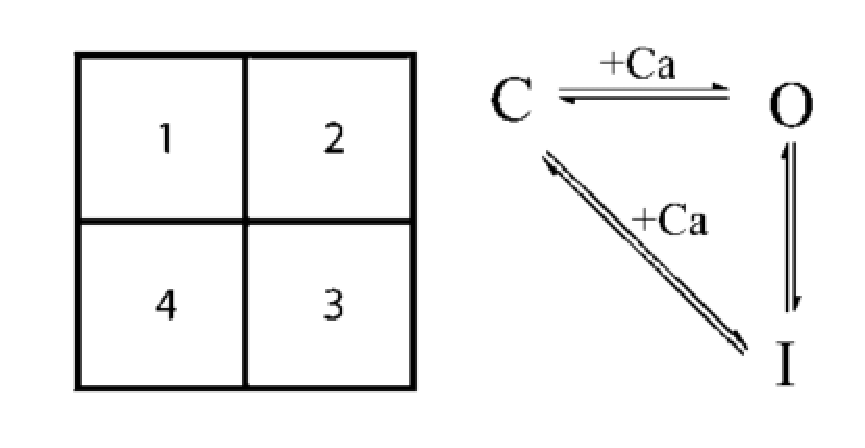
\includegraphics[height=4cm]{./images/Wang2005_RyR.eps}}
\caption{Schematic diagram of 3-state RyR subunit; and RyR tetramer}
\label{fig:Wang2005_RyR}
\end{figure}

The number of RyR tetramer in the simulation was $N_\ryr=100$ \citep{28}.
Other parameters:
\begin{enumerate}
  \item single channel conductance: $g_\ryr = 800$ per sec.
\end{enumerate}
Other assumptions: all RyRs sense the same calcium concentration $[\Ca]_\ds$.
The total flux $J_\ryr$ is proportional to the number of opening RyR:
$N_{\ryr,o}$.
\begin{equation}
J_\ryr = N_{\ryr,o}.g_\ryr.\left([Ca]_\jsr-[Ca]_\ds\right)
\end{equation}


\subsection{Groff-Smith (2008)}
\label{sec:RYR_Groff2008}

\citep{sobie2002tcas} proposed the formula for coupling based
on the number of open channel. Similarly, ~\citep{groff2008} use the similar
mean-field approach using the number of channels in a given state (close, open),
yet the coupling factor is not post-hoc, but based on the microscopic
parameters, i.e. energy interactions, and average connectivity.

Also, the transition from close to open is now assumed to be
calcium-dependent (activation) with Hill-coefficient is $\eta$, i.e. $c^\eta$.
\begin{equation}
  \label{eq:1131}
  \ce{C <=>[\ce{k^+ c^\eta \chi_C}][k^-\chi_O] O}
\end{equation}
with $\eta > 1$ (typically $\eta=2$); $\chi_C, \chi_O$ are the coupling factor
to be determined later.

There are two things we need to investigate here: (1) the effect of
calcium in the dyadic subspace, (2) the effect of allosteric coupling between
neighboring RyRs.

\subsubsection{\textcolor{red}{\bf Subspace calcium dependence}}

At first, we temporarily ignore the coupling factors so the gating is subspace
calcium dependent only $c^\eta$.
\begin{equation}
  \ce{C <=>[\ce{k^+ c^\eta}][k^-] O}
\end{equation}
If $c$ is assumed constant ($c=c_\infty$), we turn back to the well-known
telegraph process with infinitesimal generator (Q-matrix), given by
\begin{equation}
 \mathbf{Q} = \{ q_{ij}\} = \left( \begin{array}{cc}
 -k^+c^\eta_\infty & k^+c^\eta_\infty \\
  k^- & -k^- \\
 \end{array}\right)
\end{equation}

If $c$ is a time-dependent function, we can take $c^\eta$ out, and generate two
component matrices. Using Q-matrix approach, the
cluster of $N$ RyRs, say in a state configuration
$\mathbf{i}=(i_1,i_2,...,i_N)$, where $i_k$ is the state of channel
$k$-th can transit to a new state $\mathbf{j}$ with a transition rate
$q_{ij}$
\begin{equation}
  \label{eq:1137}
  \mathbf{Q} = (q_{ij}) = \mathbf{K^-}+c^\eta\mathbf{K^+}
\end{equation}

The following part describes how to calculate $c$ based on the distance
$\mathbf{r}$ to the channel mouth. At first, the calcium collected at a point is
composed of the calcium contributed from all other channels in the cluster.
Consider the cluster of $N$ RyRs in a planar bilayer
($z_n=0$), and we assume linear superposing local $[\Ca]$ increase due to the contribution of
calcium diffusing from individual (opening) RyR channels at the
release site. So, the position of the RyR $n$-th, on the planar bilayer, can be
written as $\mathbf{r}_n=x_n.i+y_n.j$. Another assumption is the single (high
concentration) $\Ca$ buffer and the buffer is mobile. Then, the
calcium concentration at an arbitrary point of coordinate
$\mathbf{r}=x.i+y.j+z.k$ is
\begin{equation}
  \label{eq:1144}
  c(\mathbf{r})=\sum^N_{i=1}\frac{\sigma_n}{2\pi|\mathbf{r}_n-\mathbf{r}|(D_c+\kappa_\infty
    D_b)}\left[1+\frac{\kappa_\infty D_b}{D_c}\exp\frac{-|\mathbf{r}_n-\mathbf{r}|}{\lambda}\right]
\end{equation}
with
\begin{eqnarray}
  \label{eq:1145}
  \frac{1}{\tau} &&= k^+_bc_\infty + k^-_b \\
  \frac{1}{\lambda^2}&&=\frac{1}{\tau}\left(\frac{1}{D_b}+\frac{\kappa_\infty}{D_c}\right)
  \\
  \kappa_\infty &&= \frac{K_b[B]_T}{(K_b+c_\infty)^2}
\end{eqnarray}
$\sigma_n$ is the source amplitude (i.e. number of $\Ca$ ions passing
through per unit of time) of the channel $n$. $D_c,D_b$ is diffusion
coefficient of free $\Ca$ and buffer, respectively. $k^+_b,k^-_b$ is
the association/dissociation constant of calcium binding. The
buffer is assumed rapid-buffering.

\begin{framed}
  The single mobile buffer is assumed Calmodulin-like buffer, i.e.
  $k^+_b=100\mu$M$^{-\eta}$.s$^{-1}$, $k^-_b=38$s$^{-1}$,
  $D_c=250\difu$, $D_b=32\difu$
\end{framed}
\begin{framed}
  There are different factors that may affect unitary RyR current,
  e.g. lumenal calcium. This lumenal calcium dependence was
  not added into the model, a phenomenon that is expected to reduce the
  effective unitary current of RyR {\it in vivo}. So, they assumed there are
  only 2 conducting states, and they are all the  same for all channel
  \begin{equation}
    \label{eq:1132}
    \sigma_n(t) = \left\{
      \begin{array}{ll}
        0 & \text{if channel open}\\
        \overline{\sigma} & \text{if channel close}
      \end{array}
    \right.
  \end{equation}
  and all channels are assumed to have the same unitary current
  \begin{equation}
    \label{eq:1133}
    \overline{\sigma} = \frac{i_\ryr}{z_\ca F}
  \end{equation}
  $i_\ryr=0.4$pA.
\end{framed}

The amount of elevated calcium contributed to a single channels, from all other
channels in the cluster can be represented in the form of a
coupling matrix C=($c_{nm}$) of size  $N\times N$, with $c_{nm}$ represents
the amount of calcium affected to channel $m$ diffused from channel
$n$ when channel $n$ opens. % Now, the location of the examining channel is consider as
% the origin, and the distance from $m$ to $n$ is $r_d$
Suppose the position of the $\Ca$ regulatory site for channel $m$ is
$r_d$ distance above the channel pore, then its position is
$a_m=x_m.i+y_m.j+r_d.k$, and the calcium elevation at that position is
\begin{equation}
  \label{eq:1147}
  c_{nm}=\frac{\sigma_\circ}{2\pi|\mathbf{r}_n-\mathbf{a}_m|(D_c+\kappa_\infty
    D_b)}\left[1+\frac{\kappa_\infty D_b}{D_c}\exp\frac{-|\mathbf{r}_n-\mathbf{a}_m|}{\lambda}\right]
\end{equation}
with $\sigma_n(t)=\sigma_\circ$ if the channel open.

So, the total calcium at the regulatory site of channel $m$ (at a distance
$a_m$ to the pore) is
\begin{equation}
  \label{eq:1148}
  c_m = c_\infty + \sum^N_{n=1} c_{nm}
\end{equation}
which is the calcium that involves in the determination of state change
of RyR $m$-th as depicted in eq.~\eqref{eq:1131}. The matrix $\mathbf{C}$
also represents the {\it coupling strength}.

\begin{framed}
  The calcium coupling strength $c_{nm}$ can be adjusted by (1)
  changing the channel source amplitude, (2) buffer parameters, or (3)
  the diffusion constant for free $\Ca$.
\end{framed}

\subsubsection{\textcolor{red}{\bf Mean-field approximation to
calcium-dependence}}

As calculating $c_m$ for every channel in the cluster is computationally
expense, ~\citep{groff2008} used a mean-field approach, i.e. the
contribution from any open channel to the neighboring one is the same,
regardless of their position. So, they proposed a formula for coupling strength
as the average of the off-diagonal elements of the coupling matrix $\mathbf{C}=(c_{mn})$.
\begin{equation}
  \label{eq:1149}
  c^* = \frac{1}{N(N-1)}\sum^N_{
    \begin{array}{l}
      n,m=1\\
      n\ne m
    \end{array}
  }
  c_{nm}
\end{equation}
which is a decreasing function of $[\BT]$ for any fixed unitary
current $i_\ryr$, and increasing function of $i_\ryr$ for fixed
$[\BT]$.

So, in the mean-field approach, each opening channel is assumed to contribute
the same amount of calcium $c^*$ to the calcium elevation of the neighboring
one, then if channel $m$ has $n$ opening neighboring channels, the level of calcium at the regulatory
site is
\begin{equation}
  \label{eq:1154}
  c_m = c_\infty + nc^*
\end{equation}

\subsubsection{\textcolor{red}{\bf Allosteric coupling}}

The microscopic term of allosteric coupling is represented via the interaction
energy $E_{ij}$ between any two channels $i$ and $j$. However, as $E_{ij}$ and $k_BT$ has the same unit
and $k_BT$ is the smallest energy discretization, instead of using free energy $E_{ij}$ as
described in ~\citep{stern1999lcm},~\citep{groff2008} defined
dimensionless free energy $\mathcal{E}_{ij}$ of interactions (in unit
of $k_BT$). Then, the new quantity of rate transition is $Q_{ij}$,
rather than $K_{ij}$.

These unitless interaction energies are organized into a matrix
$\mathcal{E}_{M\times M}$ with $M$ is the number of single-channel
states and $\varepsilon_{ij}=\varepsilon_{ji}$ ($i\ne j$) to satisfy
the requirement of thermodynamics reversibility.

Example: 2-state RyR model, i.e. $M=2$
\begin{equation}
  \label{eq:1135}
  \mathcal{E}=\left(
    \begin{array}{ll}
      \varepsilon_{CC} & \varepsilon_{CO}\\
      \varepsilon_{OC} & \varepsilon_{OO}
    \end{array}
\right)
\end{equation}

With the coupling term, so, instead of $k_{ij}$ in the component matrices, we
have the new quantities $K_{ij}$, as described in eq.~\eqref{eq:1130}. However,
as describe above, a unitless energy term is used, i.e.
\begin{equation}
  \label{eq:1139}
  K_{ij} = k_{ij} \exp\left(-\eta_{ij}\sum^4_{m=1}(\varepsilon_{js_m}-\varepsilon_{is_m})\right)
\end{equation}
with $s_m$ can be C or O in the example above. As the exponential can change
over time, to make it easier in matrix manipulation,

% Now, if we move the
% exponentia out
% combine with the calcium-dependent factor, i.e. $q_\ij = k_{ij}
% c^\eta$
\begin{equation}
  \label{eq:1151}
  \tilde{q}_{ij} = q_{ij}
  \exp\left(-\eta_{ij}\sum^4_{m=1}(\varepsilon_{js_m}-\varepsilon_{is_m})\right)
\end{equation}

Example: In the 2-state RyR model above
\begin{equation}
  \label{eq:1152}
  \begin{split}
    q_{CO} &= k^+ c^\eta\\
    q_{OC} &= k^-
  \end{split}
\end{equation}

To generalize the summation from 1 to $N$ the number of channel in the cluster,
rather than using 4 as the number of neighbors, \textcolor{red}{the adjacent
matrix} is defined as
\begin{equation}
  \label{eq:1136}
  A = (a_{mn}) = \left\{
      \begin{array}{lc}
        1 & \text{if 2 channels $m$ and $n$ are adjacent} \\
        0 & \text{otherwise} \\
      \end{array}\right.
\end{equation}
so, eq.\ref{eq:1151} can be rewritten as
\begin{equation}
\label{eq:1190}
  \tilde{q}_{ij} = q_{ij}
  \exp\left(-\eta_{ij}\sum^N_{m=1}(a_{js_m}\varepsilon_{js_m}-a_{is_m}\varepsilon_{is_m})\right)
\end{equation}
NOTE: $a_{nn}=0$, as a channel does not experience allosteric
interaction with itself.

Using matrix notation, a convenient way to formulate eq.~\eqref{eq:1190} for the
channel $n'$ from state $i$ to $j$ is
\begin{equation}
  \label{eq:1140}
  \tilde{q}_\ij = q_\ij \exp\left(-\eta_\ij(\gamma_j-\gamma_i) \right)
\end{equation}
with the total allosteric coupling energy imposing on each state is
\begin{equation}
  \label{eq:1141}
  \begin{split}
    \gamma_i = \sum^N_{k=1}a_{kn'}\varepsilon_{i k_s } ; \;\;  \gamma_j =
    \sum^N_{k=1}a_{kn'}\varepsilon_{j k_s}
  \end{split}
\end{equation}
% with $k_s$ is the state of the RyR $k$.


% Similar to~\citep{stern1999lcm}, to consider allosteric coupling, this
% transition rate is modified by a coupling factor $\chi_{ij}$
% \begin{equation}
%   \label{eq:1138}
%   \tilde{q_{ij}} = q_{ij}\chi_{ij}
% \end{equation}
% Utilize eq.~\eqref{eq:1140}, we have

\begin{framed}
  In general, $\eta_\ij$ can potentially receive different values for
  every transition $i$ to $j$. However, if we assume the transition
  rate involving the association of $\Ca$ are diffusion-limited, a channel when
  changing from C to O doesn't contribute anything to the neighbors or $\eta=0$
, i.e. the change in free energy from C to O cannot increase the on-rate of the
neighbors. Conversely, $\eta=1$ for all other configuration where channels make
O to C transition.  So, for the 2-state RyR model, using the assumption of
diffusion-limited, a cluster of $N$ channels has state transition of individual
channels
  \begin{equation}
    \label{eq:1156}
    \begin{split}
      \tilde{q}_{CO} &= k^+c^\eta \\
      \tilde{q}_{OC} &= k^-\exp(-(\gamma_2-\gamma_1))
    \end{split}
  \end{equation}
\end{framed}

\begin{enumerate}
  \item In the 2-state RyR model, using the assumption of diffusion-limited,
the allosteric energy is the combination of
$(\varepsilon_{CC}-\varepsilon_{CO})$ and
$(\varepsilon_{OC}-\varepsilon_{OO})$.

\item In the 3-state RyR model, e.g. $\ce{S1 <=> S2 <=> S3}$, using the
assumption of diffusion-limited, the allosteric energy is the combination of
$(\varepsilon_{S_1S_2}-\varepsilon_{S_1S_1})$,
$(\varepsilon_{S_1S_2}-\varepsilon_{S_2S_2})$,
$(\varepsilon_{S_1S_3}-\varepsilon_{S_1S_1})$,
$(\varepsilon_{S_1S_3}-\varepsilon_{S_3S_3})$,
\end{enumerate}
Therefore, the problem is getting much more complicated if we
consider 3-state and above. To simplify that, without the loss of generality, we
can assume that the coupling energy from a channel only favor the neighbors to
switch to the same state with it. So, we can assume
$\varepsilon_{CO}=\varepsilon_{OC}=0$ or any  $\varepsilon_{S_iS_j}=0$ with
$i\ne j$. It means we focus on the allosteric interaction that promotes
synchronous gating or it promotes the neighboring channel
to have the same state with it ($\varepsilon_{CC}\le 0, \varepsilon_{OO}\le 0$).

\begin{framed}
The experimental result showed that allosteric interaction is not
required for channel to exhibit synchronous gating. Indeed, coupled
gating can be mediated entirely via buffered diffusion of local
calcium as long as this concentration is high enough,
e.g. $c^*=0.75\mu$M. In the 2-state RyR model, optimal $c^*$ is an
increasing function of the magnitude of $\varepsilon_{CC}$. Indeed,
sparks statistics (peak, rate, duration) depend on $c^*, \varepsilon_{CC},
\varepsilon_{OO}$ in a complicated manner.
\end{framed}

Consider a pair of state transition
\begin{equation}
  \label{eq:1142}
  \begin{split}
    \tilde{q_\ij} &=q_\ij\exp\left(-\eta_\ij(\gamma_j-\gamma_i)
    \right)\\
    \tilde{q_\ji} &=q_\ji\exp\left(\eta_\ji(\gamma_j-\gamma_i)
    \right)\\
  \end{split}
\end{equation}
So, with $n_\ij=1-n_\ji$, then $1 = (n_\ij+n_\ji)$ and
\begin{equation}
  \label{eq:1143}
  \frac{\tilde{q_\ij}}{\tilde{q_\ji}} = \frac{q_\ij}{q_\ji}\exp(-(\gamma_j-\gamma_i))
\end{equation}

\subsubsection{\textcolor{red}{\bf Mean-field approximation to
allosteric-coupling}}

The current challenge is calculating eq.\ref{eq:1141}. To simplify this,
mean-field approach is utilized. In mean-field approach, we don't examine the
state transition of individual channel, but the state transition of the cluster
as a whole. In different computational studies, it was demonstrated that {\bf
mean-field approach} (i.e. ignoring the spatial arrangement of RyRs) to modeling
RyR clusters often perform well. So, ignoring the  position of individual
channels in the cluster, we can get rid of  examining the number of neighbors
(maximum 4) of a given channel to calculate  the energy contributing from these neighbors.


Even though \citep{sobie2002tcas} also used a mean-field approach, they used an
ad-hoc approach to formulate allosteric coupling
(Sect.~\ref{sec:RYR_Sobie2002}).
Here, ~\citep{groff2008} simplified Stern {\it et  al.} approach
(Sect.\ref{sec:RYR_Stern1999}) and solve it using matrix computational approach.
In particular, when the locations are not important, i.e. all RyRs are
indistinguishable, the adjacent matrix can be now mapped to a new form
$\mathbf{\overline{A}}=(a^*)$, where $0\le a^*\le 1$ is the average allosteric
connectivity
\begin{equation}
  \label{eq:1150}
  a^* = \frac{1}{N(N-1)}\sum^N_{
    \begin{array}{l}
      n,m=1\\
      n\ne m
    \end{array}
  }
  a_{nm}
\end{equation}

As described in the previous section using mean-field approach, the contribution
of calcium from one channel to its neighbor is represented in a matrix form
$\mathbf{\overline{C}} = (c^*)$. Similarly, if $N_o$ is the number of open
channel in the cluster, each channel is  assumed to have $N_o$ opening
neighbors.

\begin{framed}
  NOTE: It's impossible to generate a cluster of RyR that satisfies
  any of the two assumptions: $c^*$ and $a^*$. However, it simplifies
  dramatically the computational demand and the simulation results are
  still reasonable.
\end{framed}

When using mean-field approach, there's a change in definition of cluster state.
The old definition of a state of a cluster is
$\mathbf{i}=(s_1,s_2,...,s_N)$ in which $s_i$ is the current state of
channel $i$, $s_i=1..M$. Using mean-field approach, the new definition
of a state of a cluster is $\mathbf{\overline{i}}=(n_1,n_2,...,n_M)$, with $n_i$
is the number of channels in the cluster in state $i$.

Consider 2 cluster-states: $\mathbf{\overline{i}}=(n_1,n_2,...,n_M)$ and
$\mathbf{\overline{j}}=(n_1-1,n_2+1,...,n_M)$. So, for a transition from
cluster-state $\mathbf{\overline{i}}$ to $\mathbf{\overline{j}}$, one channel switchs from
channel-state 1 to channel-state 2. However, there are $n_1$ channels in
channel-state 1, so there are $n_1$ possibilities of selecting a channel to
change the state, i.e.
\begin{equation}
  \label{eq:1155}
  q_\ij = n_1 k^+ (c_\infty + N_O c^*)^\eta
\end{equation}
with $N_O$ is the number of open channel.

Example: Consider the 2-state RyR model above (i.e. if $N_o$ is the number of
channel in state 2 (open), then number of channel in state 1 (close) is $N-N_o$)
and using the assumptions of (1) mean-field approach, (2) calcium
diffusion-limited ($\eta_{CO}=0,\eta_{OC}=1$), and (3) the coupling favor
synchronous gatings, i.e. $\varepsilon_{CO}=\varepsilon_{OC} = 0$,  a cluster of
$N$ channels has state transition as given

\begin{equation}
  \label{eq:1153}
  \begin{split}
    \tilde{q}_{CO} &= (N-N_O)k^+(c_\infty + N_O.c^*)^\eta\\
  \tilde{q}_{OC} &= k^- N_O
  \exp\left(-a^*(-(N_O-1)\varepsilon_{OO}-(N-N_O)
    \varepsilon_{CC})\right)
%
%     \tilde{q}_{OC} &= k^- N_O
%     \exp\left(-(a^*(N_O-1)(\varepsilon_{OC}-\varepsilon_{OO})-(N-N_O)
%       a^*(\varepsilon_{CC}-\varepsilon_{CO}))\right)
  \end{split}
\end{equation}

If we relax the second condition, which is used by \citep{williams2008mclc}, we
will have
\small
\begin{equation}
  \label{eq:1153}
  \begin{split}
    \tilde{q}_{CO} &= (N-N_O)k^+(c_\infty + N_O.c^*)^\eta
    \exp\left(-a^*\eta_{CO}(-(N_O-1)\varepsilon_{OO}-(N-N_O)
    \varepsilon_{CC})\right)
    \\
  \tilde{q}_{OC} &= k^- N_O
  \exp\left(-a^*\eta_{OC}(-(N_O-1)\varepsilon_{OO}-(N-N_O)
    \varepsilon_{CC})\right)
  \end{split}
\end{equation}
\normalsize
In general, there are 9 parameters to be considered: $N$, $k^+$, $k^-$,
$\varepsilon_{OO}$, $\varepsilon_{CC}$, $a^*$, $\eta_{CO}$, $\eta_{OC}$.
\textcolor{red}{Sparks are less sensitive to variations in $c^*$, when
$\varepsilon_{CC}$ becomes more negative (i.e. coupling strength increased); and
more sensitive to variations in $c^*$, when $\varepsilon_{OO}$ becomes more
negative}.

The function being used here is analogous to the function being used by
\citep{sobie2002tcas}, i.e. $\chi_{C}$ is an increasing function of $N_c$.
However, the function being used here is non-linear and increase exponentially.

NOTE: With no allosteric interactions, $\varepsilon_{CC}=\varepsilon_{OO}=0$. For
allosteric interactions that stabilize closed channel pairs, e.g.
$\varepsilon+{CC}=-0.8$ ($k_BT$). For allosteric interactions that stabilize open
channel pairs, e.g. $\varepsilon_{OO}=-0.8$. For allosteric interactions that
stabilize both open channels pair and closed channel pairs, we can choose
$\varepsilon_{CC}=-0.8, \varepsilon_{OO}=-0.8$.

\begin{framed}
EXPLANATION: $\tilde{q}_{OC}$ is the transition from O to C. So, if there are
$N_o$ channels open, and the channel under examined is Open, there will be
$(N_o-1)$ Open neighbors and $(N-N_o)$ Closed neighbors. As a result,
\small
\begin{equation*}
\begin{split}
\tilde{q}_{OC} &=k^-N_o \exp \left(\sum \varepsilon_{Cs_m} -
\varepsilon_{Os_m}\right) \\
  &= k^-N_o \exp\left(-a^*\left(
(N_o-1) \varepsilon_{CO} +
(N-N_o)\varepsilon_{CC} - (N_o-1)\varepsilon_{OO} - (N-N_o)\varepsilon_{OC}
\right) \right)  \\
  &= k^-N_o \exp\left(-a^*\left(
(N_o-1) (\varepsilon_{CO} - \varepsilon_{OO}) +
(N-N_o) (\varepsilon_{CC} - \varepsilon_{OC})
\right) \right)  \\
\end{split}
\end{equation*}
\normalsize
\end{framed}
%
%  When we consider a channel, there is only (N-1) to be considered as
%  neighboring. It means that if the channel to be examined is Close, then under mean-field
% approach, it has $N_o$ Open neighbors, and $(N-N_o-1)$ Close neighbors. However,
% when it change from C to O, i.e. $\chi_C$, in the next state, the number of open
% channel is $(N_o+1)$ and number of close is $$

% Similarly, if the channel to be examined in Open, it has $(N_o-1)$ Open
% neighbors, and $(N-N_o)$ Close neighbors.
% \begin{eqnarray*}
% \gamma_C = \sum^N a_{k_{n'}}\varepsilon_{k_s C} = a^* ( (N_o) (\varepsilon_{OC})
% + (N-N_o-1)(\varepsilon_{CC})) \\ \gamma_O = \sum^N a_{k_{n'}}\varepsilon_{k_s
% O} = a^* ( (N_o-1) (\varepsilon_{OO}) + (N-N_o)(\varepsilon_{CO}))
% \end{eqnarray*}
% then combining with the assumption of allosteric coupling favor synchronous
% gating, i.e. $\varepsilon_{OC} = \varepsilon_{CO} = 0$
% , then
% \begin{equation}
%   \label{eq:1157}
% \end{equation}


\section{Adaptation}
\label{sec:RyR_adaptation}

To read: \citep{Velez1997}

In 1993, Gyorke and Fill showed that RyR displays ``adaptation'' in response to
successive \ce{Ca^2+} elevation~\citep{gyorke1993ryr} (The experiment was
carried under the absence of $\Mg$).
By adaptation, it means that after rapid activation by a step increase in
$[\Ca]_\ds$, the channel undergoes a slow spontaneous decrease in $P_o$.
In other words, adaption of the RyR is the subsequent decline of RyR channel
open probability $P_o$ even though $[\Ca]_\ds$ level remains constant, e.g. the
transition to state C2 from O1 as shown in Fig.\ref{fig:KeizerSmith_RyR}.
So, the channel switches to another non-conducting state, C2, but not the
Closed state. This state is denoted as ``Inactivated" state or ``adapted" state.

Another explanation is that RyR experiences a slow inactivation, i.e.
spontaneous decrease in $P_o$ after a fast activation by a step increase in
$[\Ca]$ at the cytosolic face, then the channel is ``adapted" as subsequent
increase in $[\Ca]$ produces a nearly identical rise in $P_o$.
An additional step increase of $[\Ca]_\ds$ results in an increase in open
probability to a higher level, e.g. the transition from O1 to O2. RyR activation
occur within milisecond, whereas inactivation occur on a timescale of a few
seconds. Then, during subsequent increase in $[\ce{Ca}]_i$, they produces a
nearly identical rise in the open probability.


\begin{framed}
Fast activation of \tIPthreeR by $\Ca$ and a slow inactivation by $\Ca$ is
sufficient to explain \IPthree-induced oscillation in a number of cell types
\citep{deyoung1992spip3, atri1993spm}. These oscillations can occur without
$\Ca$ influx and efflux.
\end{framed}

For \tIPthreeR, the inactivation is known $\Ca$-dependent. Structural
similarities between RYR and \tIPthreeR might suggested the same mechanism of
inactivation in RyR \citep{berridge1993}. \citep{tang1994, cheng1995}. In
opposite, \cite{keizer1996rra} prposed a model where the inactivation is not
$\Ca$-dependent (Sect.\ref{sec:keizer-levine-1996}).

At physiological level of $\Mg$, \citep{valdivia1995} found that adaptation is
faster. To account for this, we can adjust the rate constant in c stage in
Keizer-Levine (1996) model. However, the model is not suitable for stochastic
simulation, as it doesn't reproduce single channel recording. To resolve this,
\citep{keizer1998} proposed a 6-state model to replicate the open and dwell
times of isolated RyR channels in vitro and in vivo.

Other experimental results shown that adaptation is too slow to account for
termination of release \citep{valdivia1995}.

\subsection{Keizer-Levine (1996)}
\label{sec:keizer-levine-1996}

To model adaptation,~\citep{keizer1996rra} used 4 states (2 open and 2 close)
for the entire RyR rather than the individual subunits,
Fig.\ref{fig:Keizer_Levine_RyR}. Though the subunits may interact to each other,
little is known about how the subunits function \citep{ogawa1994}. The
activation is assumed to be $\Ca$-dependent, with binding of $n$ and $m$ $\Ca$
ions from C1 to O1, and O1 to O2, respectively.

\begin{figure}[hbt]
  \centerline{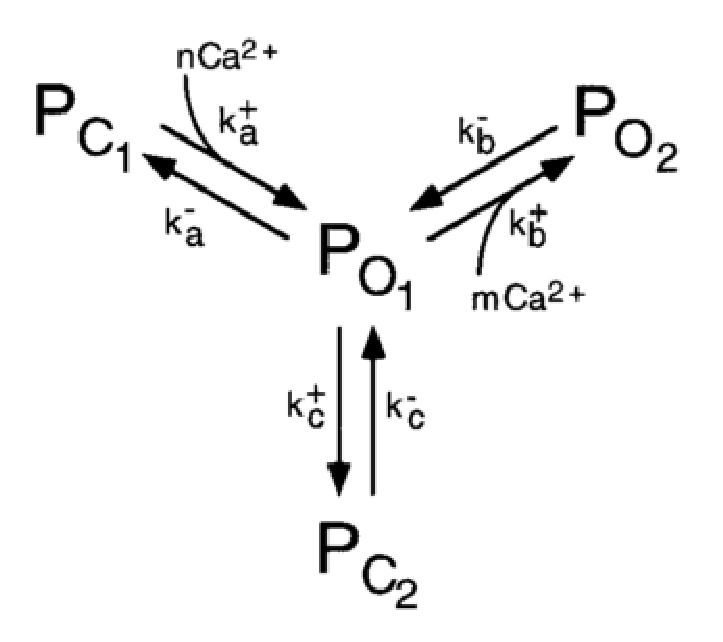
\includegraphics[height=5cm,
    angle=0]{./images/KeizerLevine_model.eps}}
  \caption{Schematic diagram of RyR. The model has 2 open states $O_1,
    O_2$ and 2 closed states $C_1, C_2$. Transitions from $C_1$ to
    $O_1$, and $O_1$ to $O_2$ are $\Ca$-dependent.}
\label{fig:Keizer_Levine_RyR}
\end{figure}

At rest (low Calcium), the channels reside primarily at C$_1$ (at basal $[\Ca] =
0.1\muM$, a small fraction of RyR still open $P_o \sim 0.01$ in the model) .
Upon calcium increase (jumping from 0.1 to 0.9$\muM$), the channels briefly
switch to O$_1$ and O$_2$ (increasing peak $P_o \sim 0.963$), allowing
\ce{Ca^2+} to be released.
This lead to the peak open probability which is followed by a decline as the
slow transition to close state C$_2$.
In the absence of the transition from O1 to C2, there's no adaptation. When the
transition between O1 and C2 are sufficiently low, the mechanism exhibits slow
inactivation. The second open state O2 is important to keep the plateau open
probability increasing as $[\Ca]$ increase.

Here, the inactivation is assumed to be $\Ca$-independent, i.e.
the transition from O$_1$ to C$_2$ is calcium-independent.
Upon additional increase of calcium level, the channel reopen by its transition
to open state O$_2$. O$_2$ is an important to the model as it help maintaining
the plateau open probability increasing as $\ce[Ca^2+]_i$ increase.

\begin{framed}
  In Keizer-Levine closed-cell kinetic model, RyR adaptation cause
  \ce{Ca^2+} oscillation in closed cell. However, {\it in vivo}, in an
  open-cell, not RyR adaptation produce \ce{Ca^2+} oscillation.
\end{framed}

Even though multiple $\Ca$ ions do not bind simultaneously to the RyR, it's
assumed that this is the case so that Hill-type approximation can be used.
\begin{equation}
\begin{split}
dP_{C1}/dt &= - k^+_a[\Ca]^n_i P_{C1} +  k^-_a P_{O1} \\
dP_{O1}/dt &= k^+_a[\Ca]^n_i P_{C1} - k^-_a P_{O1} - k^+_b [\Ca]_i^m P_{O1} +
k^-_b P_{O2} - k^+_c P_{O1} + k^-_c P_{C2} \\
dP_{O2}/dt &= k^+_b [\Ca]_i^m P_{O1} - k^-_b P_{O2} \\
dP_{C2}/dt &= k^+_c P_{O1} - k^-_c P_{C2}
\end{split}
\end{equation}\
$k^+, k^-$ and $m$, $n$	are determined by data fitting (experimental data is
from \citep{gyorke1993ryr}), Table.\ref{tab:keizer_RyR_constants}.
Qualitatively, steps a and b should be fast (miliseconds), whereas step c is slow (second time scale).
The first constraint is that
\begin{equation}
P_{C1}+P_{O1}+P_{C2}+P_{O2} = 1
\end{equation}
If we fix $[\Ca]_i$, the three equations to be resolved is linea and thus
straightforward to analyze. The fitted model is simulated in
Fig.\ref{fig:Keizer_RyR_Po}.

\begin{table}[hbt]
\begin{center}
    \begin{tabular}{lc}
        \hline
        Rate constant & Value \\
        \hline \hline
        $k^+_a$  & 1500 $\muM^{-4}.s^{-1}$ \\
        $k^-_a$ & 28.8 s$^{-1}$ \\
        $k^+_b$ & 1500 $\muM^{-3}.s^{-1}$ \\
        $k^-_b$ & 385.9 s$^{-1}$ \\
        $k^+_c$ & 1.75 s$^{-1}$ \\
        $k^-_c$ & 0.1 s$^{-1}$ \\
        \hline
    \end{tabular}
\end{center}
\caption{RyR kinetic constant (n=4,m=3)}
\label{tab:keizer_RyR_constants}
\end{table}

As $P_{C2}$ changes slower than other states, other states can reach equilibrium
before $P_{C2}$ changes appreciably.

\begin{figure}[hbt]
  \centerline{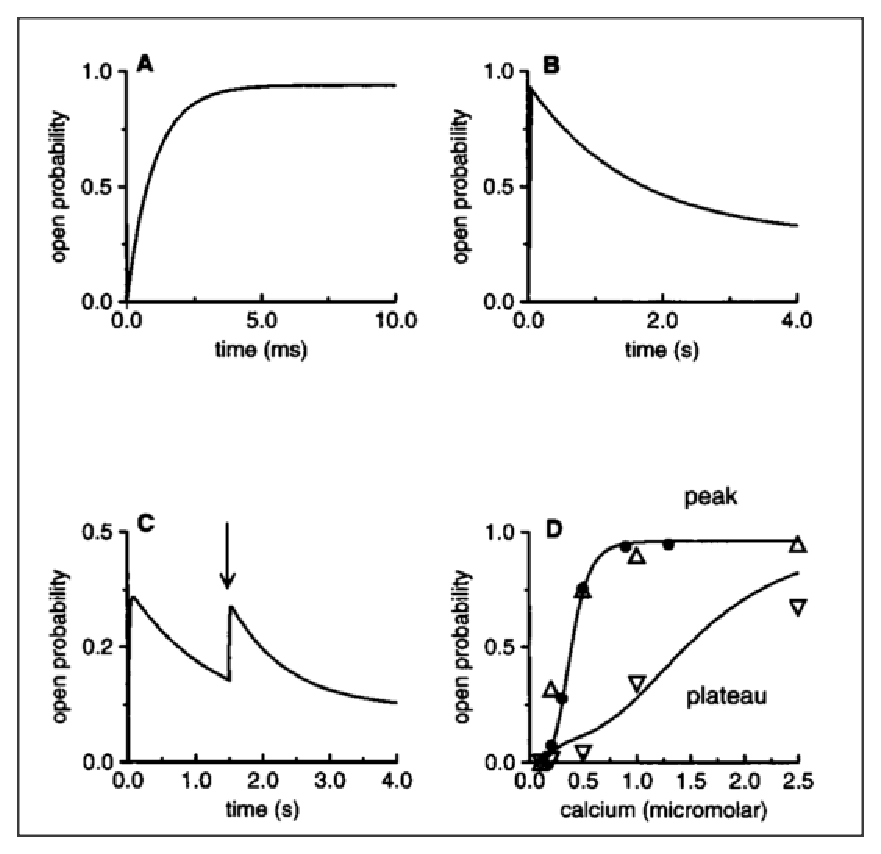
\includegraphics[height=5cm,
    angle=0]{./images/Keizer_RyR_Po.eps}}
  \caption{(A) $P_o$ of RyR when $[\Ca]_i$ increase from 0.1 to 0.9$\muM$; (B)
  similar to (A) yet with a longer time scale; (C) Two elevations of $[\Ca]$
  from 0.1 to 0.35$\muM$ at t=0; and to 0.50$\muM$ at the arrow - the adapted
  response make lesser RyR to be ready for another opening; (D) The peak and
  plateau $P_o$ as a function of $[\Ca]$ (simulation and experimental data)}
  \label{fig:Keizer_RyR_Po}
\end{figure}

At fixed $[\Ca]_i$, the rate of relaxation of $w$ determine the rate of
relaxation of $P_o$ to its plateau value (in the model, the relaxation time is
1.0sec for $[\Ca]_i = 0.5\muM$, 1.9sec for $[\Ca]_i = 1.0\muM$, and 2.0sec for
$[\Ca]_i = 0.2\muM$)
\begin{equation}
dw/dt = - \frac{(w - w^\infty)}{\tau}
\end{equation}
with $w^\infty( [\Ca]_i)$ and $\tau([\Ca]_i)$ are equilibrium value and
relaxation time, both function of $[\Ca]_i$.

 At higher $[\Ca]_i > 5\muM$, the plateau rise somewhat higher
(1.0 rather than 0.75). This can be resolved by ading another closed state C$_3$, connected to
C$_2$ by $\Ca$-dependent transition. This has not been added into the model.
Also, the model lacks to reproduce the rapid ``flickering'' of the channel in
open state. Also, stochastic simulation doesn't guarantee to reproduce all the
detailed transitions observed in single-channel currents.




\subsection{Keizer-Smith (1998)}
\label{sec:Keizer-Smith_98}

\citep{keizer1998} proposed a 6-state model to replicate open and dwell-times of
isolated RyR channels in vitro and in vivo, as well as measured peak and plateau
open probabilities with $\Ca$ and cesium $\Cs$ as the charge carrier,
Fig.\ref{fig:KeizerSmith_RyR}. So, so transition rates depend on $[\Ca]$ in the
microdomain, while some depend on $[\Ca]$ in the bulk myoplasm.

\begin{figure}[hbt]
  \centerline{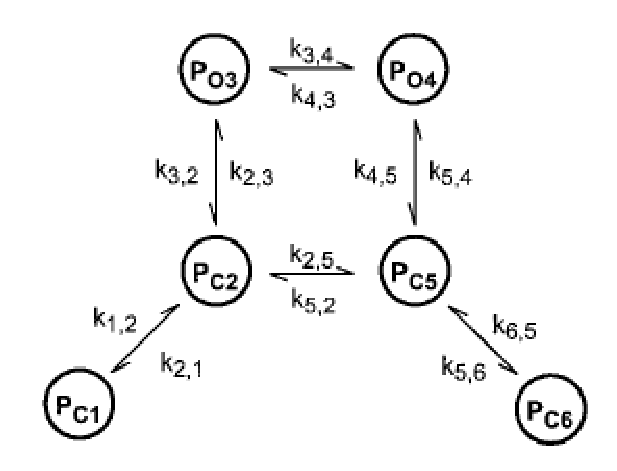
\includegraphics[height=5cm]{./images/KeizerSmith_RyR.eps}}
\caption{Schematic diagram of a RyR}
\label{fig:KeizerSmith_RyR}
\end{figure}

$P_{C1}, P_{C2}$ represent the initial closed states. With the increase in
$[\Ca]_\ds$, the channels open, transiting to state $P_{O3}, P_{O4}$. States
$P_{C5}, P_{C6}$ represent {\it adaptation} and {\it refractory} state.


\subsection{Greenstein-Winslow (2002)}
\label{sec:greenstein_winslow_RyR}

A 4-state model reduced from 6-state RyR model of \citep{keizer1998} was
developed \citep{greenstein2002}. The model is built when subspace calcium is $>
36.85 \muM$.

\begin{figure}[hbt]
  \centerline{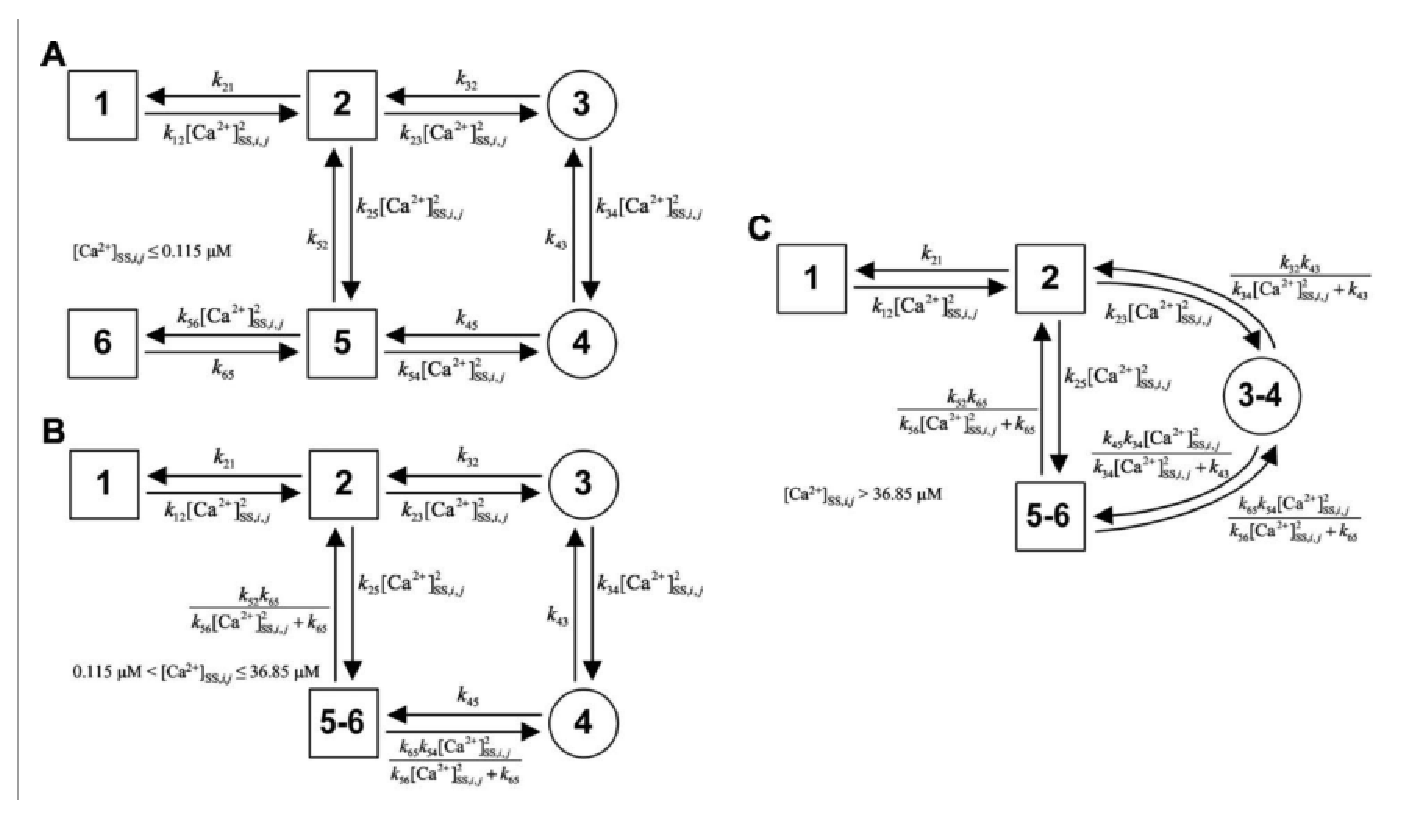
\includegraphics[height=5cm]{./images/greenstein_RyR.eps}}
\caption{RyR 4-state}
\label{fig:greenstein_RyR}
\end{figure}




\section{jSR depletion}

jSR depletion, which occurs during $\Ca$ release, may contribute to the
termination of $\Ca$ spark, by reducing $P_o$ of RyR via luminal
calcium-dependent activation. It's suggested that all the
above mechanisms could contribute to the termination of calcium sparks
\citep{sobie2002tcas}.

Models that incorporate lumenal calcium dependence are:
\citep{sobie2002tcas, williams2008mclc, williams2011}.



\section{Tang and Othmer (1994)}

The model of the ryanodine receptor (RyR) channel (Tang
and Othmer 1994) has 4 states, with 2 calcium binding sites:
\begin{enumerate}
  \item Open state R10* : only excitatory site is calcium bound
  
  \item 3 others are Closed states:
  \item R00 : calcium binding site is unoccupied
  \item R01 : inhibitory calcium binding site is occupied
  \item R11 : both calcium binding sites are occupied
\end{enumerate}

\begin{verbatim}
R00 <=>[M_2 * Ca2+] [L_2] R01 
R00 <=>[M_1 * Ca2+] [L_1] R10*
R11 <=>[L_2] [M_2 * Ca2+] R10*
R11 <=>[L_1] [M_1 * Ca2+] R01	
\end{verbatim}


\section{Snyder et al. (2000) - CSQ}
\label{sec:RYR_Snyder2000_CSQ}

\citep{snyder2000mmc} (Sect.\ref{sec:snyder_2000}) introduced CSQ as an
intermediate player that provide a bidireciontal feedback on RyR gating.
CSQ is known to be localized in the terminal cisternal portion of the SR and how
it regulates RyR2 was not clearly understood at that time. However, there are
evidences that CSQ appears forming a complex with junctin and triadin and
to attach to the junctional face membrane in the close proximity to the RyR2s
\citep{zhang1997, brandt1990}.

In skeletal muscle, efflux rate of calcium under CICR form a bell-shaped as a
function of cytosolic side free calcium, with peak at pCa = 6, and decreasing on
both side with pCa = 9 or 3. In cardiac SR, it's also a biphasic function of
free cytosolic calcium with maximum at $[\Ca]$ = 5-20$\muM$
\citep{Coronado1994}. This was hypothesized with two cytosolic $\Ca$ binding
sites: one fast-site for opening and slow-site for closing. However, this is not
necessarily calcium-binding, yet it can be $\Ca$/CaM; and the reducing in
calcium flux can also be explained by the decreasing in gradient between the
lumenal and cytosolic side. Also, there are evidences against
cytosolic $\Ca$-dependent inactivation of RyR \citep{Liu2013}.

Snyder et al. assumed calcium binding
\begin{equation}
\begin{split}
\ce{Ca^2+ + S_i <-> Ca^2+S_i} \\
\ce{Ca^2+S_i + Ca^2+ <-> (Ca^2+)_2S_i} \\
\ldots \\
\ce{(Ca^2+)_{n-1}S_i + Ca^2+ <-> (Ca^2+)_nS_i} \\
\end{split}
\end{equation}
In this case, there are two binding sites: $S_1$ and $S_2$, with 2 calcium
bindings to activate $S_1$ and only one calcium binding to activate $S_2$.

Instead of simulating individual channel, using deterministic approach, the
number of channels was mapped to concentration so that the fraction of channels
in each state is simulated. So, with the assumption of about 1.6$\times 10^6$
RyR2 per cell, the converted concentration is $0.15\muM$.
Snyder {\it et al.} assumed 4 states of RyR
\begin{enumerate}
  \item Activable: no $\Ca$ binding
  \item Open: two $\Ca$ bind to fast site with the first one is rate-limiting
  step, and enhance the second binding step which is almost in equilibrium
  ($[(\Ca)_2 S_1]]\gg [\Ca S_1]$).
\begin{equation}
\ce{Ca^2+ + S_1 <=>[k^+_1][k^-_1] Ca^2+S_i <=>[Kd(\Ca)] (Ca^2+)_2S_1 }
\end{equation}
then the new backward rate if the second phase is fast
\begin{equation}
k_r = \frac{(k^-_1)^2}{k^+_1[\Ca]}
\end{equation}
and
\begin{equation}
\frac{d[(\Ca)_2 S_1]}{dt} = k^+_1 [\Ca]_\ds ([S_1]_T - [(\Ca)_2 S_1]) - k_r
 [(\Ca)_2 S_2]
\end{equation}
with $k^+_1 = 2000$ $(\muM.s)^{-1}$.


  \item Closed: one $\Ca$ bind to fast site, one $\Ca$ bind to slow site

  \item Refractory: one $\Ca$ bind to slow site

\begin{equation}
\frac{d[\Ca S_2]}{dt} = k^+_2 [\Ca]([S_2]_T - [\Ca S_2]) - k^-_2 [\Ca S_2]
\end{equation}
with $k^+_2 = 13$ $(\muM.s)^{-1})$.

If we map $[\Ca S_2]$ to the fractional concentration of bound sites, i.e.
cas$_2$ $\in [0,1]$, then $[S_2]_T = 1$ and
\begin{equation}
\frac{dcas_2}{dt} = k^+_2 [\Ca] (1 - cas_2) - k^-_2 [\Ca S_2]
\end{equation}
\end{enumerate}

\begin{framed}
The rate of binding ions to proteins is in the range 1-3000 $(\muM.s)^{-1}$
\citep{Moore1984}.  The value $k^+$ (or $k_{on}$) in a ligand binding involving
enzymes. The value given in Snyder et al. was based on Arrhenius expression
using a diffusion-controlled reaction, in an encounter distance of $5\times
10^{-8}$ cm, and diffusion coefficient $79 \mum^2/s$ \citep{marcus1997}.

The value of $k^-$ (or $k_{off}$) is determined based on $K_d$ or $K_{CM}$ equal
to $k^+/k^-$.
\end{framed}

Using deterministic method, the fractional of RyR2 in each state is then given
by the formula
\begin{equation}
\begin{split}
r_a = (1-cas_1)(1-cas_2) \\
r_o = cas_1 (1-cas_2) \\
r_c = cas_1 cas_2 \\
r_r = (1-cas_1) cas_2
\end{split}
\end{equation}


\subsection{CSQ on RyR}

The binding of $\Ca$ to CSQ was represented using ODE, rather than instantaneous
\begin{equation}
\frac{d[\CaCSQ]}{dt} = k^+_{CSQ} [\Ca] (B_\jsr - [\CaCSQ]) - k^-_{CSQ} [\CaCSQ]
\end{equation}
The maximum buffer $B_\jsr = 0.008$ mol/(L SR water), which is in the range
0.005-0.014 mol/(L SR water) given by \citep{bers1993rrd, shannon1997}. The
buffer dissociation constant $K_{m,\jsr}=638\muM$. The buffer on-rate
$k^+_{CSQ} = 0.008772 (\muM.s)^{-1}$ was obtained from \citep{Donoso1995}.

\citep{gilchrist1992icd} demonstrated that SR would not release $\Ca$ when below
a threshold level of luminal $\Ca$. One possible explanation is that RyR2-CSQ
control loop produces an inhibitory feedback when the SR $\Ca$ load is
sufficiently reduced. A bidirectional feedback mechanism was proposed:
\begin{enumerate}
  \item Positive feedback: Binding of $\Ca$ to the RyR2 fast site induces SRRC
  to undergo a conformational change to the open state. When RyR opens, it affect RyR-CSQ
  complex in such a way that it shifts CSQ-$\Ca$ binding curve, i.e. increasing
  $K_d$ of CSQ-$\Ca$ binding constant. It means more free calcium available that
  can be released via RyR.

  \item The negative feedback: The dissociation of $\Ca$ from CSQ makes CSQ
  undergoes conformational change, which then affect RyR-CSQ complex in such a
  way that decrease $\Kd$ of $\Ca$-affinity to the RyR closing site, i.e.
  bringing $P_o$ of RyR down.
\end{enumerate}

However, Snyder et al. didn't model this bidirectional effect as an incremental
change over a range, but as a step change at the mid-value
\begin{itemize}
  \item When $[\Ca]_\jsr < 500\muM$: $k^+_2$ get 10x bigger.
  \item When $P_o$ of RyR increases ($>0.15$): $k^-_{CSQ}$ reduce 20x
\end{itemize}

% \begin{enumerate}
%   \item When $\Ca$ binds to fast-binding site on RyR, it trigger RyR opens.
%   As RyR-CSQ forms a complex, RyR opens (i.e. when fraction of RyR in open
%   state $> 0.15$) cause CSQ to change its conformation, which makes $\Kd$ of
%   $\Ca$ to CSQ increases (i.e. 20x increase), leaving more free $\Ca$ to be
%   released via RyR.
%
%   \item At a certain amount ($[\Ca]_\jsr < 500\muM$), new conformation of CSQ
%   affect RyR closing site, i.e. decreasing $\Kd$ with $\Ca$  ($K_d =  10 \times
%   k_{on,fast}$) makes $\Ca$ can easily bind to the closing site of RyR and
%   reducing RyR $P_o$.
% \end{enumerate}


Now, the role of CSQ to RyR2 was mapped to the calcium affinity on the cytosolic
side. \textcolor{red}{This is controversal, as how CSQ from the lumenal side
affect to cytosolic side of RyR2?}.

The opening of a few RyR2s is enough to cause a reduction in CSQ $\Ca$ affinity,
giving more free calcium or increase the free calcium gradient between the jSR
and the subspace.

\subsection{Calcium flux}

The flux of calcium release is then modelled using $r_o$ and passive flux
formula
\begin{equation}
J_\ryr = r_o v_\ryr ([\Ca]_\jsr - [\Ca]_\ds)
\end{equation}
with $v_\ryr = 9$ (s$^{-1}$) is the rate constant analogous to the collective
conductance of RyR2, i.e. the ease of $\Ca$ movement through the entire set of
cell's RyRs. The value measured by Kim et al. (1983) was 2-139 (s$^{-1}$)
\citep{Kim1983} and measured by Donoso et al. (1995) was 2-12 (s$^{-1}$)
\citep{Donoso1995}.

The calcium efflux
\begin{equation}
J_\ef = v_\ef ([\Ca]_\ds - [\Ca]_\myo)
\end{equation}
with $v_\ef = 2500$ s$^{-1}$. This value can be estimated using equation given
by \citep{Chen1997} for flux through channel described by unimolecular reaction
\begin{equation}
v_\ef = \frac{D_j}{d^2}\Prob \left( \text{cytosol} | \text{subspace} \right)
\end{equation}
with $D_j$ is 2D-diffusion constant in aqueous solution (which is 70$\mum^2/s$
to 79$\mum^2/s$), $d$ is the length of the channel or in this case is the
movement length of calcium from subspace to cytosol (which is $d=200$nm). They
estimated the $\Prob\left( \text{cytosol} | \text{subspace} \right)$ using
volume fractions $=\frac{V_\myo}{V_\myo+V_\ds}$

\section{Saftenku-Williams-Sitsapesan (2001)}
\label{sec:RYR_Saftenku2001}

\citep{saftenku2001} described the gating behavior of a single cardiac RyR2,
using maximum likelihood analysis to estimate the single channel kinetic
parameters. The Markovian model that reported rank highest, based on Schwartz
criterion is shown in Fig.\ref{fig:RYR_Saftenku2001}.



\begin{figure}[hbt]
  \centerline{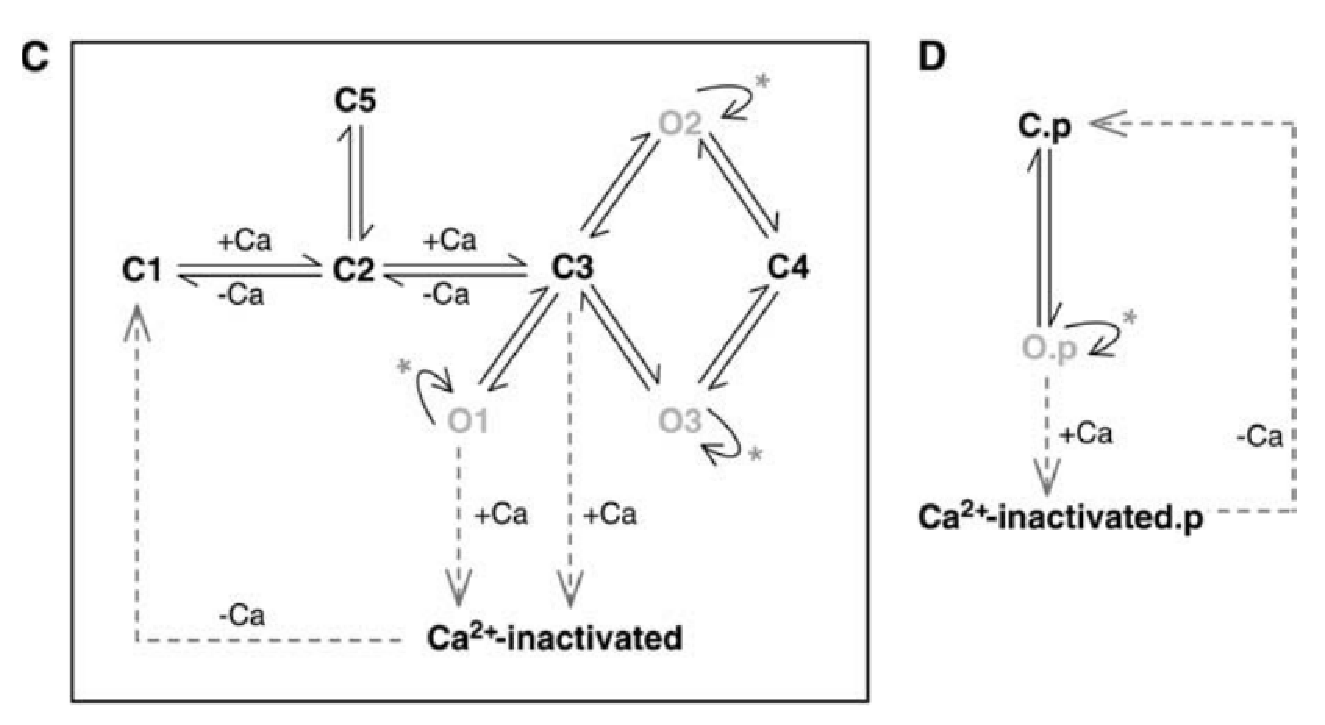
\includegraphics[height=5cm]{./images/RYR_Saftenku2001.eps}}
\caption{Schematic diagram of RyR model of 9 states}
\label{fig:RYR_Saftenku2001}
\end{figure}


The closed states are C1-C5; and open states are O1-O3. The implementation of
$\Ca$-dependent inactivation is depicted in dotted lines. This happens when
$\Ca$ binds to state O1 or C3. The choice of these two states are handpicked.
The effect of RyR2 phosphorylation is given in
Fig.\ref{fig:RYR_Saftenku2001}(B).

\section{Shannon et al. (2004)	}
\label{sec:RyR_Shannon2004}

\citep{shannon2004} extended the 4-state RyR model from Stern et al.
\citep{stern1999lcm} by adding lumenal calcium depenedent activation and
inactivation, Fig.\ref{fig:RyR_Shannon2004}.

\begin{figure}[hbt]
  \centerline{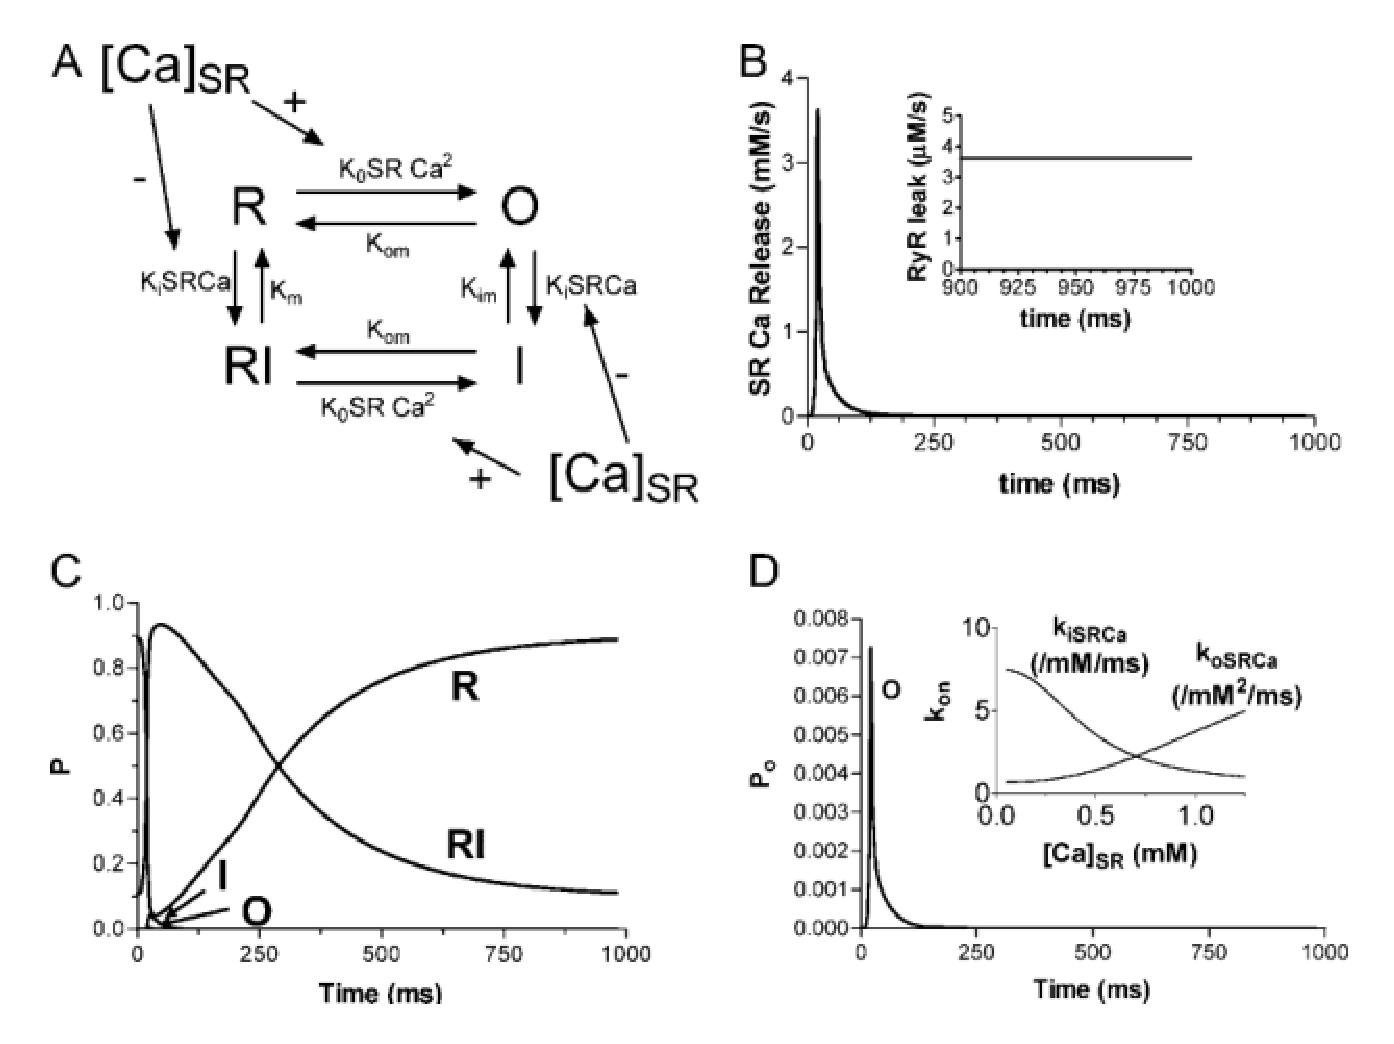
\includegraphics[height=7cm,
    angle=0]{./images/RyR_Shannon2004.eps}}
\caption{(A) Markovian model of the RyR with SR $\Ca$ dependent added, (B) SR
$\Ca$ release flux via SERCA pump backflux and RyR $\Ca$ leak (inset); (C)
Profile of 4 individual state over the course of an AP; (D) $P_o$ of RyR and
(inset) changes in $k_{on}$ with $[\Ca]_\jsr$}
\label{fig:RyR_Shannon2004}
\end{figure}

\section{Tanskanen-\ldots-Winslow (2007)}
\label{sec:Tanskanen_2007_dyad}

Typically, calcium in the dyad is represented in terms of concentration (from
0.1$\mu$M to 150$\mu$M). However, \citep{tanskanen2007} claimed that even at
peak of the spark, i.e. 150$\mu$M, this number is equivalent to a small number
of free $\Ca$ ions, i.e. $\sim 10-100$ ions. So, they suggested that modeling
calcium dynamics in the dyad using law of mass action is inappropriate.



\section{Faber-Rudy (2007)}

\citep{faber2007DHPR} introduced 10-state Markov model, modified from
\citep{fill2000}.

\begin{figure}[htb]
  \centerline{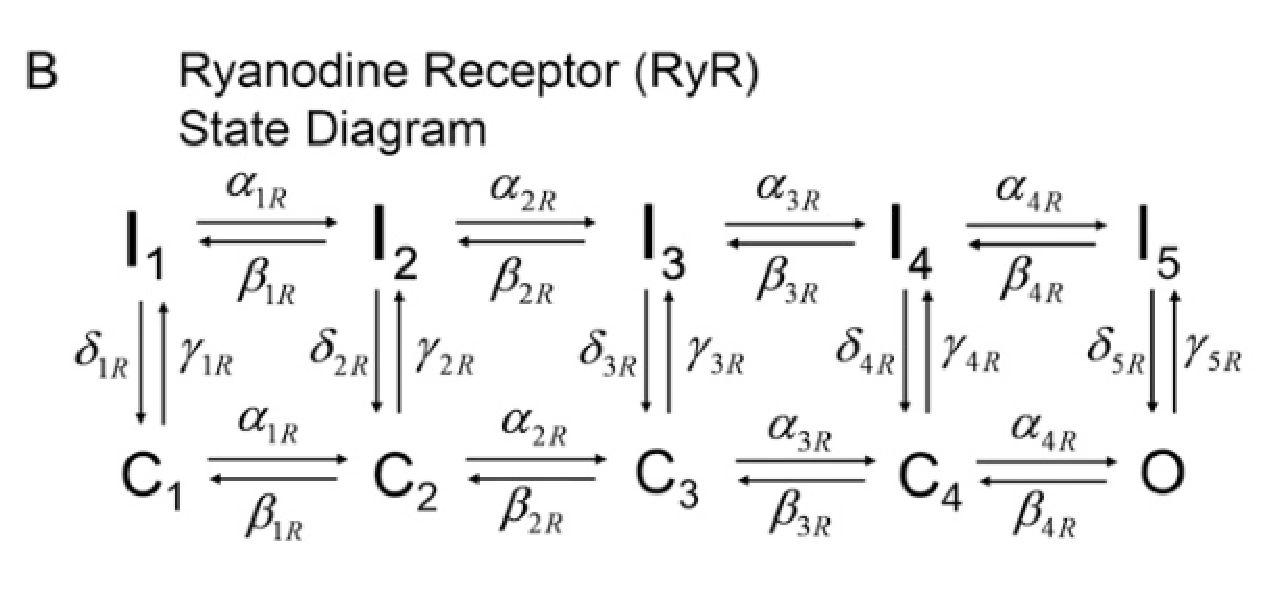
\includegraphics[height=5cm]{./images/RYR_Faber2007.eps}}
  \caption{RYR model}
  \label{fig:RYR_Faber2007}
\end{figure}


\section{Williams et al. (2008)}
\label{sec:williams-et-al-1}

~\citep{williams2007pda, williams2008mclc} modified the Groff-Smith approach
by (1) using both subspace calcium and lumenal calcium dependent of RyR
activation, (2) relaxing the assumption of calcium diffusion limited and using
$\eta_{CO}=\eta_{OC}=0.5$. The two-state model is given
as
\begin{equation}
  \label{eq:1217}
  \ce{S_i <=>[\ce{k^+.c^\eta.\phi.\chi_\ij}][\ce{k^-\chi_\ji}] S_j}
\end{equation}
% The transition rate
% $\chi_{12}=\chi_{C,O}=\chi'_C$ and $\chi_{21}=\chi_{O,C}=\chi'_O$ are
% defined as
Then, the two equations are
\begin{equation}
  \label{eq:1124}
  \chi'_C = \exp\left\{-a^*\eta_C\left[N^C_\ryr \mathcal{E}_{C,C} - (N^O_\ryr-1)\mathcal{E}_{O,O}\right]\right\}
\end{equation}
and
\begin{equation}
  \label{eq:1125}
  \chi'_O = \exp\left\{-a^*\eta_O\left[N^O_\ryr \mathcal{E}_{O,O} - (N^C_\ryr-1)\mathcal{E}_{C,C}\right]\right\}
\end{equation}
with $a^*$ is the average allosteric connectivity (based on a $7\times
7$ grid with nearest neighbor coupling. Blair et al. use
$\eta_{C}=\eta_O=0.5$. NOTE: $\eta_{C}=\eta_{CO}, \eta_{OC}=\eta_O$


\begin{itemize}
\item $\mathcal{E}_{C,O}$ is the changes of dimensionless free energy
  experienced by a channel in state C when allosterically coupled to a
  channel in state O.

\item without loss of generality, $\mathcal{E}_{C,O} =
  \mathcal{E}_{O,C}=0$. It means that there is no change in free
  energy when a channel couple to another one in a different state.

\item Instead of using the summation inside the exponential term, a
  partition allosteric coupling term is incorporated $N^C_\ryr$ and
  $N^O_\ryr$ in the mean-field approach.
  \begin{itemize}
  \item $N^C_\ryr$ = number of closed RyRs

  \item $N^O_\ryr$ = number of opening RyRs
  \end{itemize}
\end{itemize}


The sum of allosteric interaction energy between the RyR with
nearest-neighboring RyR (in the present state) is counted. This approach has
been used in \citep{williams2011}.


\section{Restrepo-Weiss-Karma (2008) - CSQ}
\label{sec:RYR_Restrepo2008-CSQ}

\citep{restrepo2008cmm} built a model to show that RyR gating mediated by CSQ
can cause calcium transient alternans (CTA)
(Sect.\ref{sec:restrepo-weiss-karma}). Here, they assume CSQ can be binding or
unbinding to RyR. \textcolor{red}{However, in many experiments, CSQ always bind
to RyR under the 0-2mM range; i.e. unbinding may occur at very high
$[\Ca]_\jsr \approx 5$mM which is beyond the physiological range}.

As CSQ can form oligomers, in this model, the binding of CSQ to RyR2 is assumed
only for CSQ monomer. The authors claimed that this simple binding model is
enough to capture the general features of CSQ modulation of RyR activity. When
a spark occurs, lumical $[\Ca]$ decreases, and then fraction of monomer M
increases. The monomers then can bind to triadin-1/junctin (T/J) complex of the
RyR channels and the fraction of CSQN-bound RyR channel increases. These
CQN-bound RyR channels have lower $P_o$, terminating the sparks.

CSQ monomer (M) form dimer (D) based on the dimerization reaction
\begin{equation}
\ce{ M + M <=>[k_1][k_2] D}
\end{equation}
Assuming of fast equilibrium, we have [M]$^2 \frac{k1/k2}=$[D], with
$\rho=k1/k2$ is a function of lumenal calcium concentration.

A crucial feature is that the transition rate from CSQN-unbounded to CSQN-bound
state depend dynamically on luminal $\Ca$ concentration through the dependence
of monomer concentration $[M]$ on $c_\jsr$.

\section{Lee-Keener (2008): RyR-CSQ}
\label{sec:RyR_Lee2008}

\citep{Lee2008} introduced the first model that incorporate CSQ into RyR gating.
They claimed that the model produce nonlinear relationship between fractional SR
$\Ca$ release and SR $\Ca$ load.

\textcolor{red}{Drawback}: (1) deterministic simulation using master equation to
determine RyR $P_o$ rather than use fully stochastic model; (2) no graded response (as a
single LCC is used only).

The activation of RyR requires binding of 2 $\Ca$ ions, while the inactivation
is the result from binding of a single $\Ca$ ion to the inactivation site of
RyR. In this model, the role of triadin and junctin is ignored, and it's assumed
that CSQ interact directly with RyR. Then, RyR is modeled with 3 binding sites:
one for CSQ, one for $\Ca$ binding activation, and one for $\Ca$ binding
inactivation.

\begin{figure}[hbt]
  \centerline{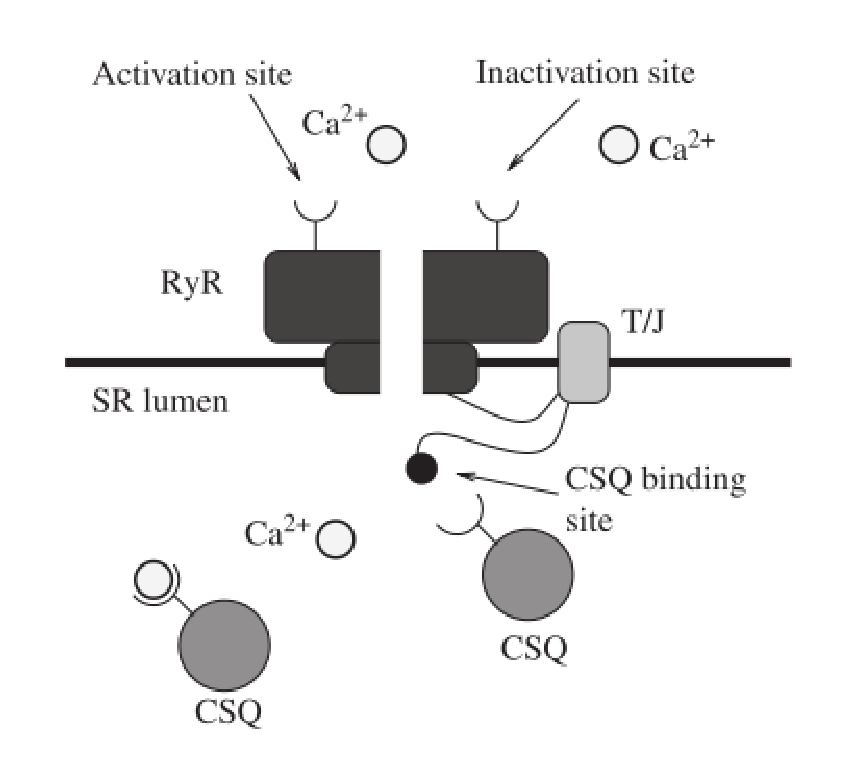
\includegraphics[height=5cm]{./images/RyR_scheme_Lee2008.eps}}
    \centerline{\includegraphics[height=5cm]{./images/RyR_8state-4state_Lee2008.eps}}
    \caption{A schematic diagram of RyR model. (B) $c$ and $q$ represent cytosolic
$\Ca$ and free $[\CSQ]$. Here, the two states enclosed in the same dotted-line
bounding box have the same cytosolic binding states}
\label{fig:RyR_scheme_Lee2008}
\end{figure}

With a state is denoted as $S_{ijk}$ with $i,j,k=0,1$ ($i$ represents CSQ
binding, $j$ represents $\Ca$ activation binding, and $k$ represents $\Ca$
inactivation binding), RyR model has 8 states. Using deterministic approach with
master equation, the fraction of channels in each state is used as a dependent
variable, i.e. $x_{ijk}$ is the fraction of RyR channels in state $S_{ijk}$.


However, the authors then reduced to 4 states as there are not enough data to
estimate all the binding rate constants for CSQ-RYR and $\Ca$-RYR interactions.
It is assumed that the association/disassociation between CSQ and $\Ca$ or RyR
are faster than $\Ca$ binding to the activation or inactivation sites of RyR.
So, on the time-scale of $\Ca$ binding, CSQ is always at quasi-steady state. So
a 4-state model is created by lumping every two states in the same dotted-line
bounding box into one. So the new fraction of channels in the 4 states are
\begin{equation}
\begin{split}
\bar{x}_{00} = x_{100} + x_{000} \\
\bar{x}_{10} = \\
\bar{x}_{01} = \\
\bar{x}_{11} =
\end{split}
\end{equation}



\section{Liang-Hu-Hu (20007, 2009)}
\label{sec:RyR_Liang2007_2009}

The rise-time (RT) has a weak dependence on the RyR cluster size, or other RyR
modulator (e.g. ATP from 0.5-5mM show little effect on RT, increase in $\Mg$
decrease spark rate but not RT). As the rise-time is quite consistent at
different conditions, it's the mechanism of spark termination that is under
investigation.

It was proposed that constant coupling (CC) lead to prolonged opening of RyR
\citep{marx2001}. A dynamic coupling (CC) was proposed which changes accordingly
to RyR functional state \citep{Liang2007}. Here, the inter-RyR coupling strength
is strong at rest to stabilize RyR in closed state, and decrease when RyR opens
to facilitate the rapid termination of $\Ca$ release.

\citep{Liang2007, Liang2009} proposed 4-state RyR, with $\Ca$ play both
activation and inactivation of RyR activity.


There are two options:
DC model and CC model.

\begin{enumerate}
  \item DC model: the coupling energy is reduced with the activation of RyR
  channels.
  \item CC model: the ecoupling energy has no dependency on channel functional
  states
\end{enumerate}


\section{Hashambhoy-Grenstein-Winslow (2010) - CaMKII phosphorylation in canine
ventricular myocyte}
\label{sec:RyR_CaMKII_Hashambhoy}

``leaky" RyR is one of the recently hypothesis to account for diminished SR
$\Ca$ level. The leaky RyR is enhanced under phosphorylation condition, e.g.
PKA-mediated or CaMKII-mediated.

\citep{Hashambhoy2010} proposed a CaMKII-RyR interaction model in canine
ventricular myocyte, with the assumption that under CaMKII phosphorylation,
$\Ca$ sensitive of RyR is increased. This model is based on CaMKII-DHPR
interaction model proposed by \citep{Hashambhoy2009}.

\section{Tania-Keener (2010): RyR-CSQ}
\label{sec:Tania-Keener_2010}

Calsequestrin (CSQ) can serves as a calcium buffer (to maintain a low level of
free $\Ca$), or modify RyR's kinetics (by binding to intrinsic SR membrane
proteins Triadin-1 and Junctin) (See Sect.\ref{sec:CSQ}).

\subsection{Hypotheis analysis}
\label{sec:tania_2010_hypo-analysis}

\citep{tania2010} derived the method proposed by Hinch \citep{hinch2004mag,
hinch2005} to develope a mechanistic 2-state stochastic process of RyR-CSQ interaction
using several asymptotic approximations and mean first exit time calculation
from the master equations. Even though the approximate behavior of a single RyR
cluster is induced, there's no assumption that channels acts as one mega-channel
as being used in \citep{hinch2004slc, williams2007pda}.

The full 6-state model is given in Fig.\ref{fig:Tania_RyR-CSQ}. When $[\Ca]_\ds$
is low, channel is in the closed state $C_1$. With more $\Ca$, 4 $\Ca$ ions can
bind to the channel, bringing it to state $C_2$, and then to the conducting
state O. Now to model the effect of CSQ, we mirror the states into 2 modes: B
(CSQ-bound), and U (CSQ-unbound). $q$ is the concentration of CSQ.

\begin{figure}[hbt]
 \centerline{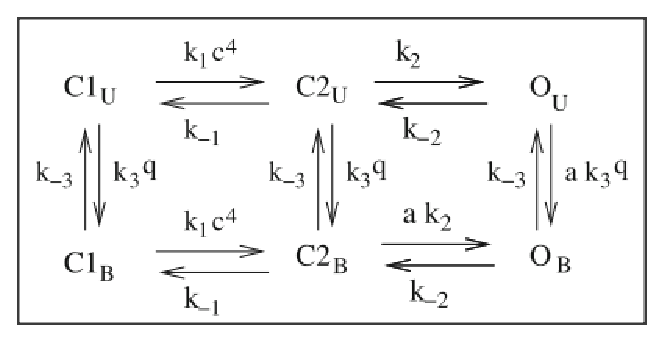
\includegraphics[height=5cm]{./images/Tania_RyR_CSQ.eps}}
\caption{Markov model of RyR-CSQ interaction}
\label{fig:Tania_RyR-CSQ}
\end{figure}

As luminal calcium ($[\Ca]_\sr$) change the channel activity by changing the
opening probability, not the open time duration \citep{gyorke1998}, the authors
assumed CSQ also have the same effect, so they derive 2 modes with Bound mode
the rate to opening is lower. This is modeled by multiplying the opening rate by
a constant $a < 1$. To preserve the detail-balance, the rate from $O_U$ to $O_B$
is multiplied by $a$ as well.

Using another assumption: fast binding/unbinding of both $\Ca$ and CSQ to RyR,
the 6-state model can be reduced to 2-state model.
\begin{enumerate}
  \item $O_U$ and $O_B$ to O
  \item $C_{1U}$ and $C_{1B}$ to $C_1$
  \item $C_{2U}$ and $C_{2B}$ to $C_2$
  \item $C_1$ and $C_2$ to $C$.
\end{enumerate}

\subsection{Purpose}

Study the effect of changing CSQ expression on calcium release profile, i.e.
spark duration, rate and critical SR $\Ca$ level for calcium release
termination.

\section{Gaur-Rudy (2011)}
\label{sec:RyR_Gaur2011}

\citep{Gaur2011} developed a RyR model with gating is a function of both $\Ca$
and CSQ, Fig.\ref{fig:RyR_Gaur2011}. RyR has 4-state with two tier of
mode-gating (upper and lower). The upper tier is called activatio tier, and the
lower one is called refractory tier. In the lower tier, $K_m$ for $\Ca$
activation is 10x higher than the upper tier (i.e. 150$\muM$ vs. 15$\muM$). The
transition from one tier to another is a function of CSQ.

NOTE: \textcolor{red}{Lumenal $\Ca$ dependent of RyR2 gating is assumed
exclusively via CSQ}.

\begin{figure}[hbt]
  \centerline{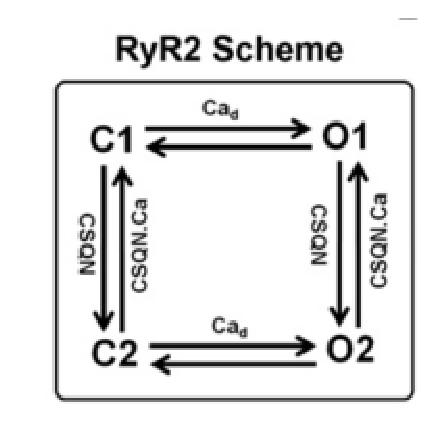
\includegraphics[height=4cm,
    angle=0]{./images/RyR_Gaur2011.eps}}
\caption{RyR scheme}
\label{fig:RyR_Gaur2011}
\end{figure}

Assumption:
\begin{enumerate}
  \item $\Ca$ binding to CSQ is instantaneous. [CSQ] is 10mM, with $K_d = 0.8$
  mM.
  \item
\end{enumerate}

\section{Laver-\ldots-Cannell (2012)}
\label{sec:RyR_Laver2012}

\citep{laver2012} measured RyR mean opening and closed time ($\tau_\open$,
$\tau_\close$, respectively). Arranging RyR in a planar lipid bilayers in the
presence of physiological levels of $\Mg$ and ATP. In particular, 230mM
$\ce{CsCH3O3S}$, 20mM CsCl (pH=7.4), with 2mM ATP and 3mM $\ce{MgCl2}$ on the
cytoplasmic side.

The open probability $P_o$ is small (0.001) at 10$\muM$ and increase to the peak
$\sim 0.5$ at 100$\muM$ of calcium (the model shown it stay at this level for
15ms before RyRs start to close when luminal $[\Ca]_\jsr$ drop to 10\% of
resting levels).
The closure of RyR was completed in $\sim 22$ms.  The dependency on luminal
calcium is due to the interactions between RyR calcium flux and
luminal/cytoplasmic $\Ca$ sensing sites \citep{laver2008}.
However, the effect is modest \citep{laver2007}.
The dependency of $P_o$ and $\tau_\close$ on $[\Ca]$ follow a non-linear
function of power 2.8 for $[\Ca]$ between 10 and 100$\muM$, i.e.
$f([\Ca]^{2.8})$.

RyR gating is modeled with 2-minimal state stochastic model with opening and
closed rate was determined from experimental data. The transition rate is given
as a function of subspace calcium with the power 2.8 for activation and -0.5 for
inactivation
\begin{equation}
\ce{\text{Close} <=>[k^+][k^-] \text{Open}}
\end{equation}
with
\begin{equation}
\begin{split}
k^+ = \min\left\{ 600, 3.17\times 10^5 \times ([\Ca]_\ds)^{2.8} \right\} \\
k^- = \max\left\{ 500, 158 \times ([\Ca]_\ds)^{-0.5} \right\}
\end{split}
\end{equation}


%%% Local Variables: 
%%% mode: latex
%%% TeX-master: "mainfile"
%%% End: 
